\documentclass{article}

\usepackage{fancyhdr}
\usepackage{extramarks}
\usepackage{amsmath}
\usepackage{amsthm}
\usepackage{amsfonts}
\usepackage{tikz}
\usepackage[plain]{algorithm}
\usepackage{algpseudocode}
\usepackage{mathtools}
\usepackage{graphicx}
\graphicspath{ {./Images/} }

\DeclarePairedDelimiter\abs{\lvert}{\rvert}%
\DeclarePairedDelimiter\norm{\lVert}{\rVert}%

\makeatletter
\let\oldabs\abs
\def\abs{\@ifstar{\oldabs}{\oldabs*}}
%
\let\oldnorm\norm
\def\norm{\@ifstar{\oldnorm}{\oldnorm*}}
\makeatother

\newcommand*{\Value}{\frac{1}{2}x^2}%

\usetikzlibrary{automata,positioning}

%
% Basic Document Settings
%

\topmargin=-0.45in
\evensidemargin=0in
\oddsidemargin=0in
\textwidth=6.5in
\textheight=9.0in
\headsep=0.25in

\linespread{1.1}

\pagestyle{fancy}
\lhead{\hmwkAuthorName}
\chead{\hmwkClass\ (\hmwkClassInstructor\ \hmwkClassTime): \hmwkTitle}
\rhead{\firstxmark}
\lfoot{\lastxmark}
\cfoot{\thepage}

\renewcommand\headrulewidth{0.4pt}
\renewcommand\footrulewidth{0.4pt}

\setlength\parindent{0pt}

%
% Create Problem Sections
%

\newcommand{\enterProblemHeader}[1]{
    \nobreak\extramarks{}{Problem \arabic{#1} continued on next page\ldots}\nobreak{}
    \nobreak\extramarks{Problem \arabic{#1} (continued)}{Problem \arabic{#1} continued on next page\ldots}\nobreak{}
}

\newcommand{\exitProblemHeader}[1]{
    \nobreak\extramarks{Problem \arabic{#1} (continued)}{Problem \arabic{#1} continued on next page\ldots}\nobreak{}
    \stepcounter{#1}
    \nobreak\extramarks{Problem \arabic{#1}}{}\nobreak{}
}

\setcounter{secnumdepth}{0}
\newcounter{partCounter}
\newcounter{homeworkProblemCounter}
\setcounter{homeworkProblemCounter}{1}
\nobreak\extramarks{Problem \arabic{homeworkProblemCounter}}{}\nobreak{}

%
% Homework Problem Environment
%
% This environment takes an optional argument. When given, it will adjust the
% problem counter. This is useful for when the problems given for your
% assignment aren't sequential. See the last 3 problems of this template for an
% example.
%
\newenvironment{homeworkProblem}[1][-1]{
    \ifnum#1>0
        \setcounter{homeworkProblemCounter}{#1}
    \fi
    \section{Problem \arabic{homeworkProblemCounter}}
    \setcounter{partCounter}{1}
    \enterProblemHeader{homeworkProblemCounter}
}{
    \exitProblemHeader{homeworkProblemCounter}
}

%
% Homework Details
%   - Title
%   - Due date
%   - Class
%   - Section/Time
%   - Instructor
%   - Author
%

\newcommand{\hmwkTitle}{Homework\ \#1}
\newcommand{\hmwkDueDate}{January 21, 2020}
\newcommand{\hmwkClass}{Physics 926}
\newcommand{\hmwkClassTime}{}
\newcommand{\hmwkClassInstructor}{Professor Ken Bloom}
\newcommand{\hmwkAuthorName}{\textbf{Robert Tabb}}

%
% Title Page
%

\title{
    \vspace{2in}
    \textmd{\textbf{\hmwkClass:\ \hmwkTitle}}\\
    \normalsize\vspace{0.1in}\small{Due\ on\ \hmwkDueDate\ at 5pm}\\
    \vspace{0.1in}\large{\textit{\hmwkClassInstructor\ \hmwkClassTime}}
    \vspace{3in}
}

\author{\hmwkAuthorName}
\date{}

\renewcommand{\part}[1]{\textbf{\large Part \Alph{partCounter}}\stepcounter{partCounter}\\}

%
% Various Helper Commands
%

% Useful for algorithms
\newcommand{\alg}[1]{\textsc{\bfseries \footnotesize #1}}

% For derivatives
\newcommand{\deriv}[1]{\frac{\mathrm{d}}{\mathrm{d}x} (#1)}

% For partial derivatives
\newcommand{\pderiv}[2]{\frac{\partial}{\partial #1} (#2)}

% Integral dx
\newcommand{\dx}{\mathrm{d}x}

% Alias for the Solution section header
\newcommand{\solution}{\textbf{\large Solution}}

% Probability commands: Expectation, Variance, Covariance, Bias
\newcommand{\E}{\mathrm{E}}
\newcommand{\Var}{\mathrm{Var}}
\newcommand{\Cov}{\mathrm{Cov}}
\newcommand{\Bias}{\mathrm{Bias}}

\begin{document}

\maketitle

\pagebreak

\begin{homeworkProblem}
	Express the gravitational constant in natural units. What are the associated energy, length, and time scales? These are collectively known as the Planck scale, at which gravitational interactions become important relative to the other interactions.
	\\
	\\
\textbf{Solution}
\\
\\
\[
	G=6.674\times 10^{-11} \frac{m^3}{kg\cdot s^2}
\]
First find m, kg, and s in natural units, then plug them into the definition for G.
\\
\\
Seconds:
\[
	\begin{split}
	\hbar=&6.582\times 10^{-25} GeV\cdot s=1 \\
	\Rightarrow 1s=&\frac{GeV^{-1}}{6.852\times 10^{-25}} \\
	=&1.519\times 10^{24}GeV^{-1}
	\end{split}
\]
Meters:
\[
	\begin{split}
	c=&2.998\times 10^8 m\cdot s^{-1} =1\\
	\Rightarrow 1m=&\frac{s}{2.998\times 10^8} \\
	=&\frac{1.519\times 10^{24}GeV^{-1}}{2.998\times 10^8} \\
	=& 5.067\times 10^{15}GeV^{-1}
	\end{split}
\]
Kilograms:
\[
	\begin{split}
	\hbar=&1.055\times 10^{-34}kg\cdot m^2 \cdot s^{-1} =1\\
	\Rightarrow 1kg=&\frac{s}{1.055\times 10^{-34}m^2} \\
	=& \frac{1.519\times 10^{24}GeV^{-1}}{(1.055\times 10^{-34})(5.067\times 10^{15}GeV^{-1})^2} \\
	=&5.608\times 10^{26} GeV
	\end{split}
\]
Now, back to G to plug in the values just calculated:
\[
	\begin{split}
	G=&6.674\times 10^{-11} \frac{m^3}{kg\cdot s^2} \\
	=&\frac{(6.674\times 10^{-11})(5.067\times 10^{15}GeV^{-1})^3}{(5.608\times 10^{26}GeV)(1.519\times 10^{-1})^2} \\
	=&6.710\times 10^{-39}GeV^{-2}
	\end{split}
\]
From here, just take $\sqrt{G}$ to find the length and time scales:
\[
	\begin{split}
	\sqrt{6.710\times 10^{-39}GeV^{-2}}=&8.191\times 10^{-20}GeV^{-1} \\
	=&1.62\times 10^{-35}m \\
	=&5.39\times 10^{-44}s
	\end{split}
\]
For energy, take $1/\sqrt{G}$
\[
	\begin{split}
	\frac{1}{\sqrt{6.710\times 10^{-39}GeV^{-2}}} = 1.221\times 10^{19}GeV	
	\end{split}
\]

\end{homeworkProblem}

\pagebreak

\begin{homeworkProblem}
Look up the lifetimes of these unstable particles: $\mu^-,\tau^-,K^+,\pi^+,\pi^0,\rho^0,D^+,B^+,$ and $J/\psi$. On the basis of the lifetimes, what interactions are responsible for the decays?
\\
\\
\textbf{Solution}
\\
\\

	\begin{center}
	\begin{tabular}{ c c c }
	Particle & Lifetime (s) & Interaction \\ 
	$\mu^-$ & $2.2\times 10^{-6}$ & Weak \\  
	$\tau^-$ & $2.9\times 10^{-13}$ & Weak \\  
	$K^+$ & $1.2\times 10^{-8}$ & Weak \\  
	$\pi^+$ & $2.6\times 10^{-8}$ & Weak \\  
	$\pi^0$ & $8.5\times 10^{-17}$ & EM \\  
	$\rho^0$ & $4.5\times 10^{-24}$ & Strong \\  
	$D^+$ & $1.0\times 10^{-12}$ & Weak \\  
	$B^+$& $1.6\times 10^{-12}$ & Weak \\  
	$J/\psi$ & $7.2\times 10^{-21}$ & Strong/EM \\  
	\end{tabular}
	\end{center}


\end{homeworkProblem}

\pagebreak

\begin{homeworkProblem}
Draw Feynman diagrams for the following weak decays: \(\tau^-\rightarrow \mu^-\bar{\nu}_\mu\nu_\tau, \Lambda\rightarrow pe^-\bar{\nu}_e,K^0\rightarrow \pi^+\pi^-,\Sigma^-\rightarrow n\pi^-\). And do the same for these strong decays: \(\omega^0\rightarrow \pi^+\pi^-\pi^0,\rho^0\rightarrow \pi^+\pi^-,\Delta^-\rightarrow n\pi^-\).
\\
\\
\textbf{Solution}
\\
\\
Look at figures \ref{start} to \ref{end}, you'll see the diagrams.
\\
\\

\begin{figure}[h]			
	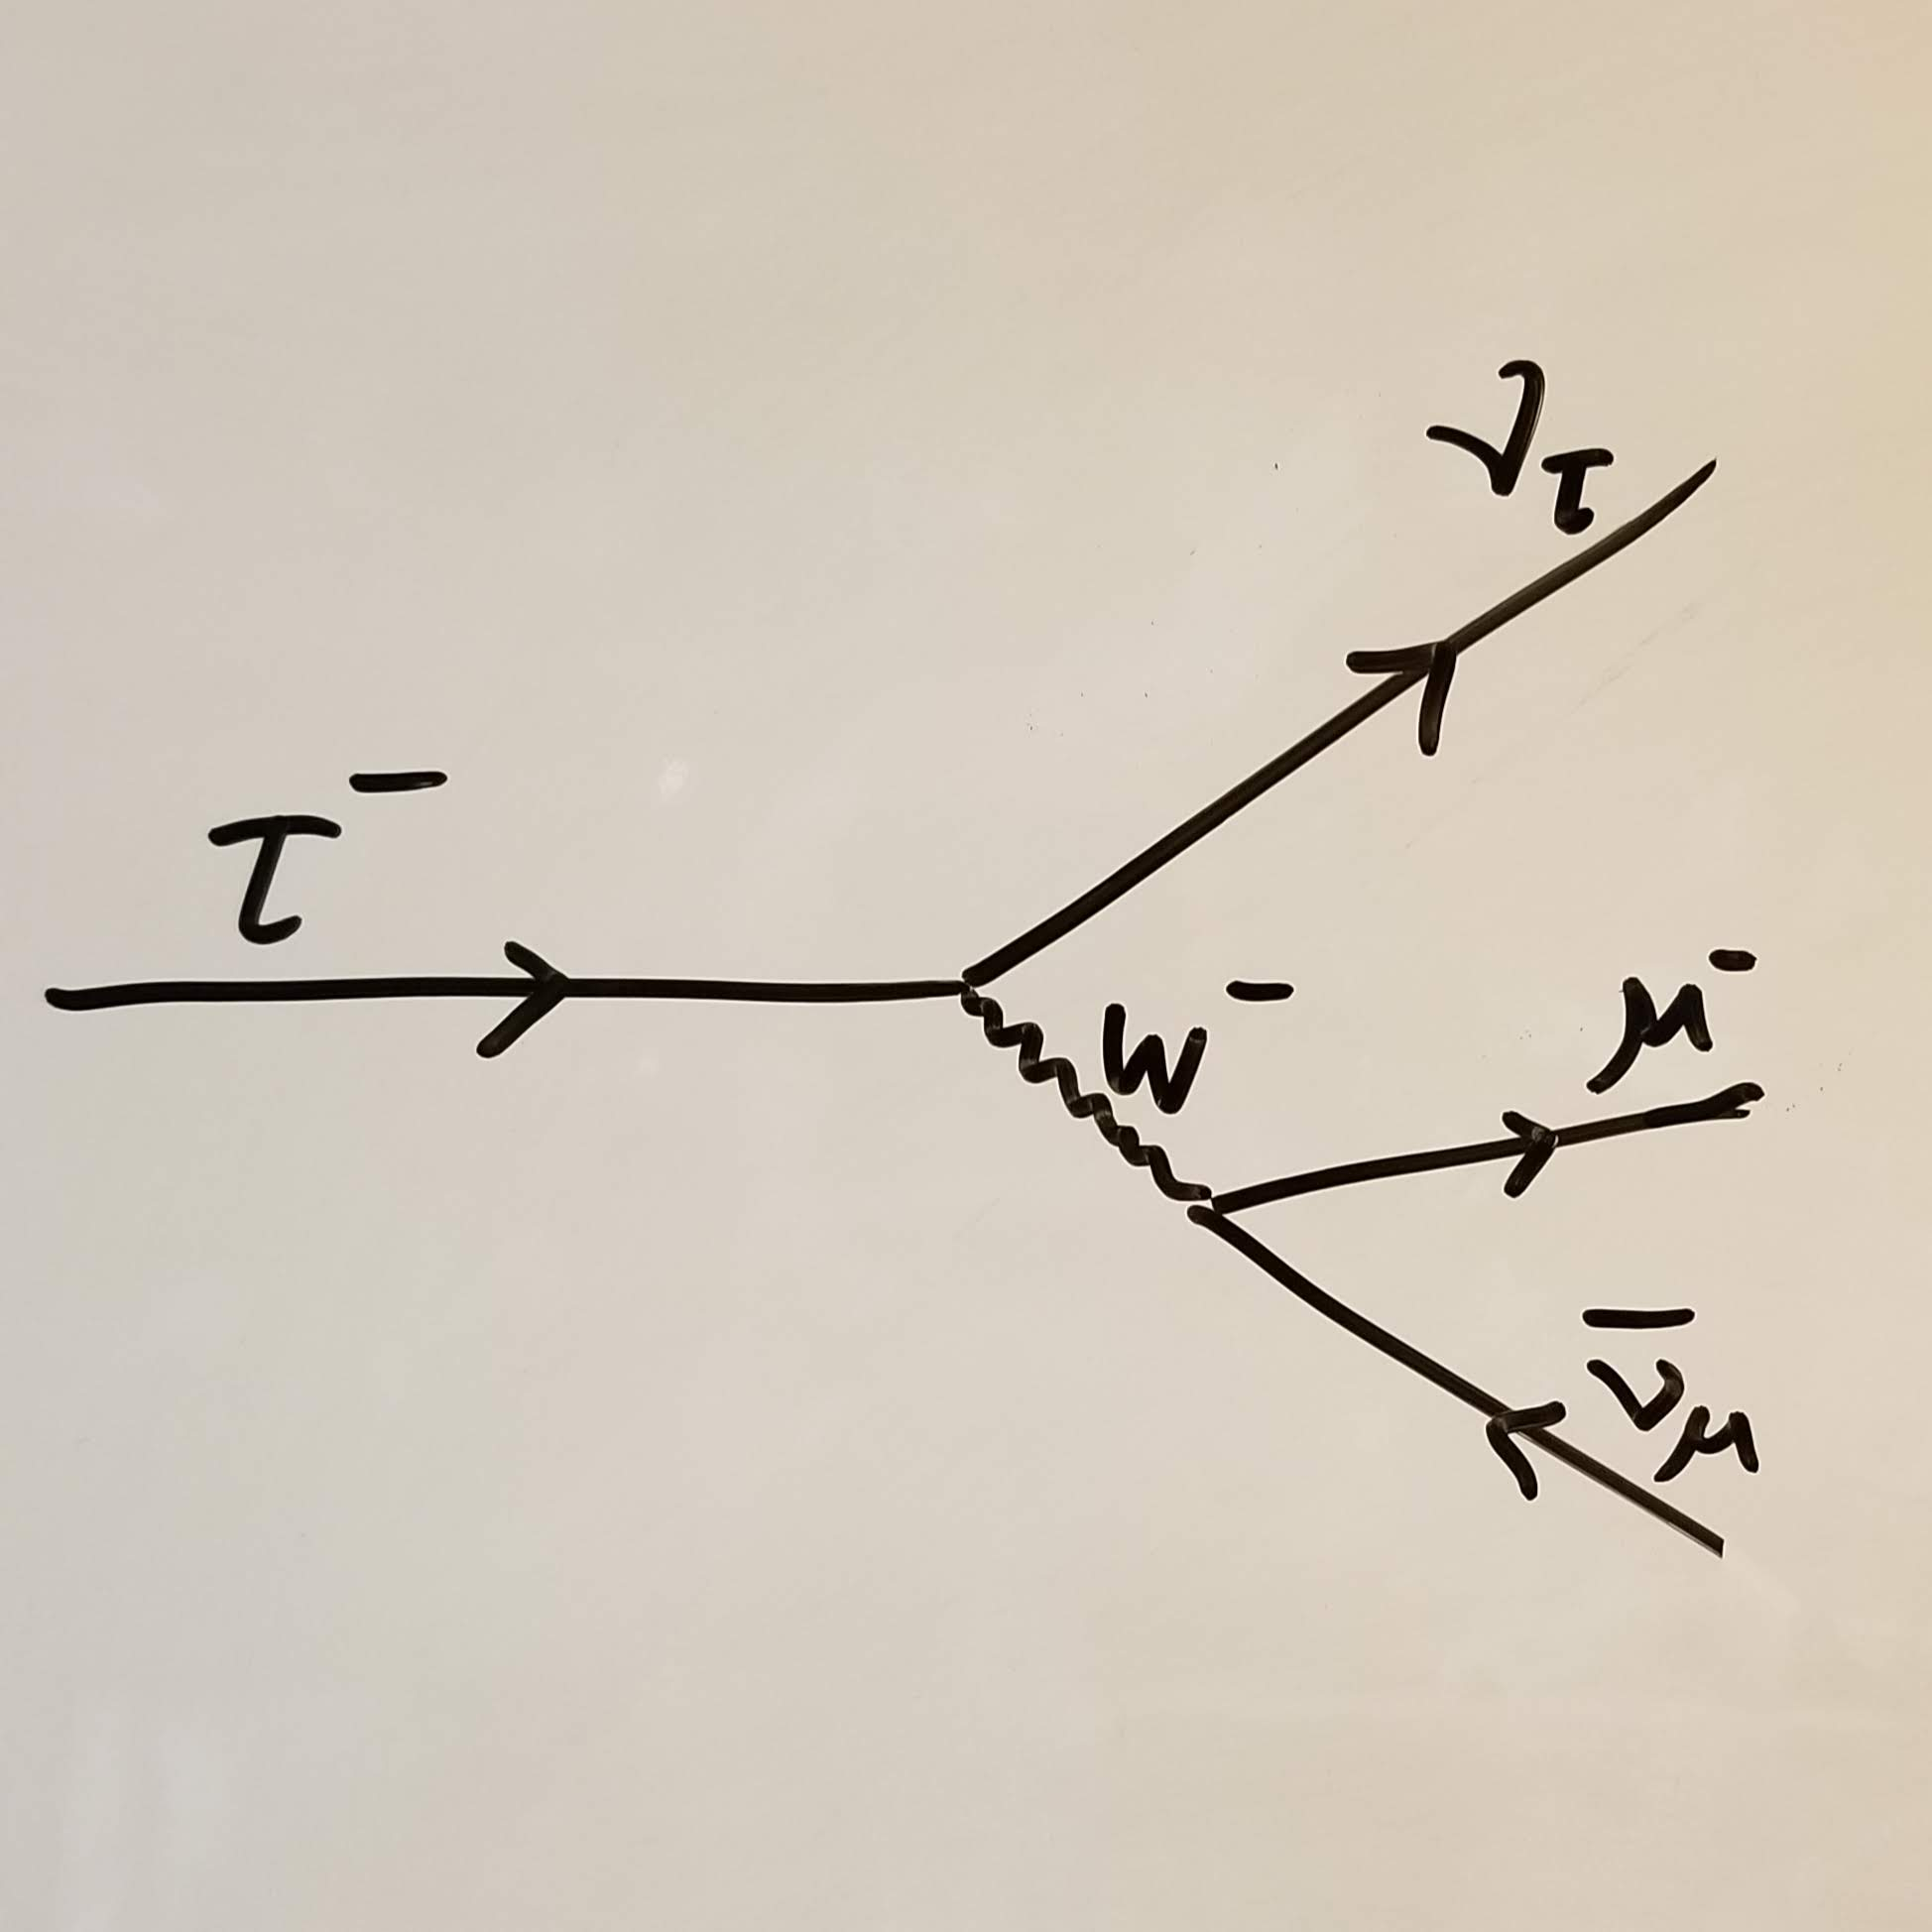
\includegraphics[scale=0.2]{tau}
	\centering
	\caption{$\tau^-\rightarrow \mu^-\bar{\nu}_\mu\nu_\tau$}
	\label{start}
	\centering
\end{figure}
\begin{figure}[h]			
	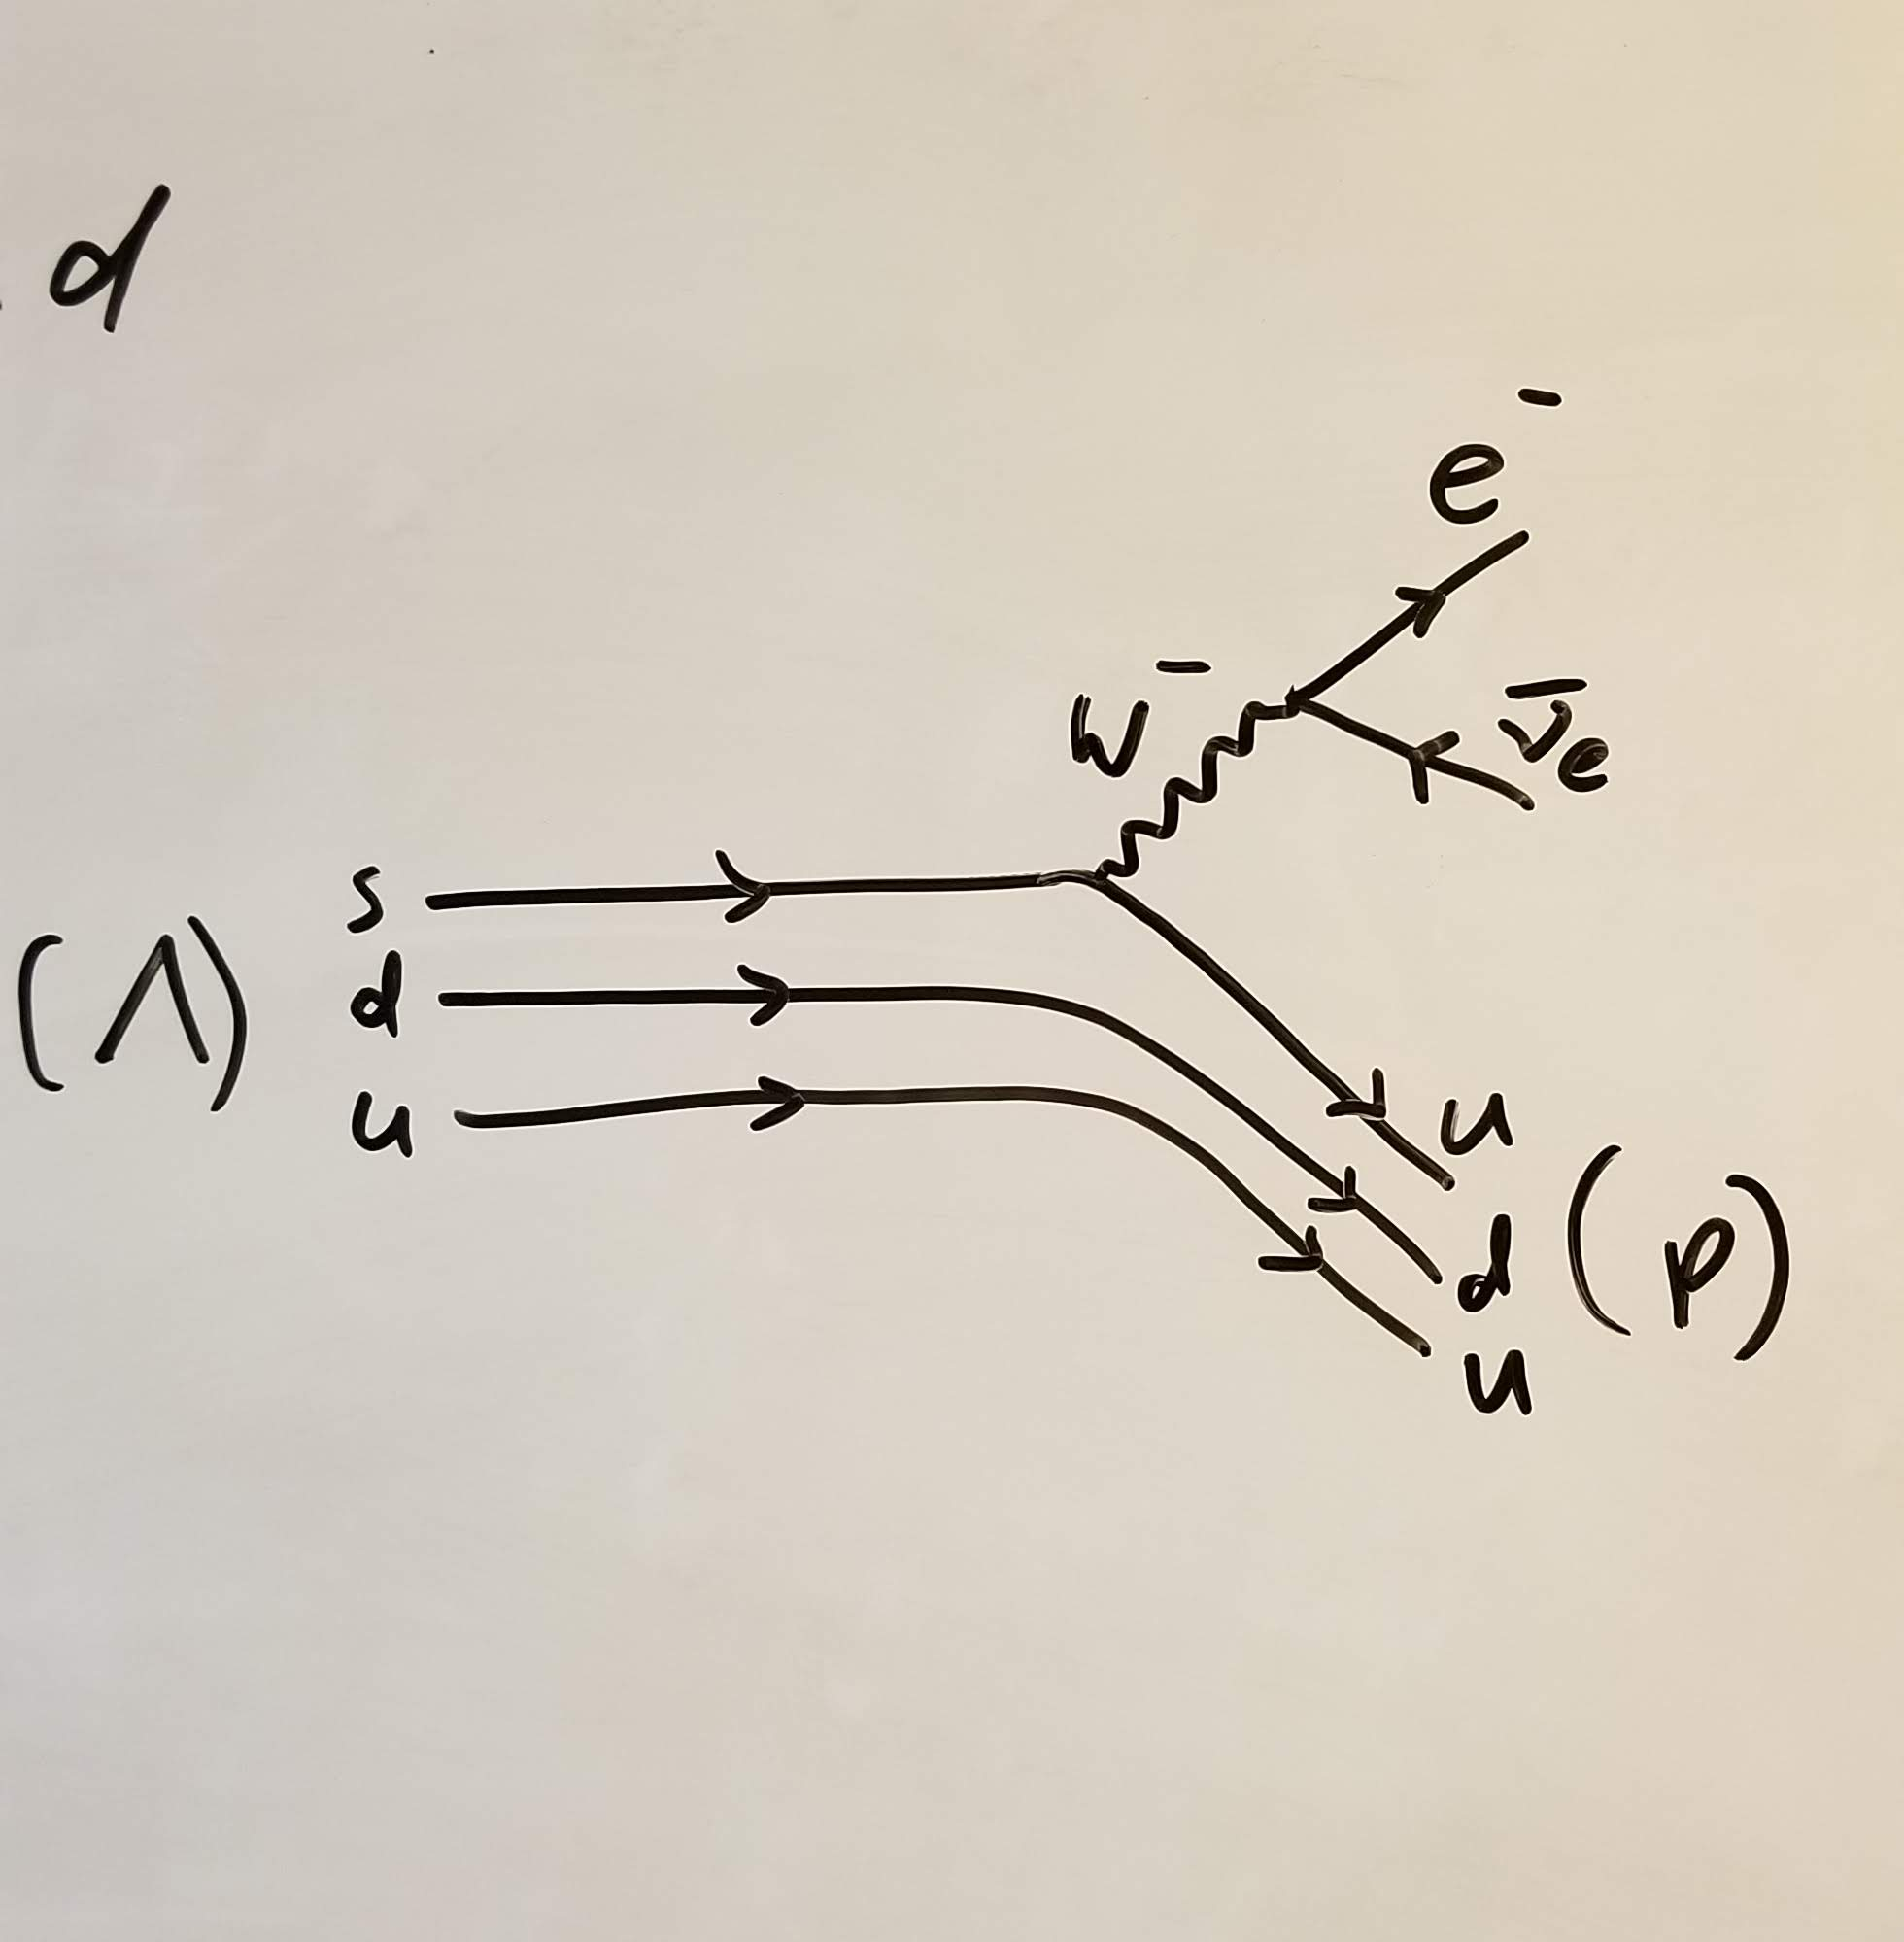
\includegraphics[scale=0.2]{lambda}
	\centering
	\caption{$\Lambda\rightarrow pe^-\bar{\nu}_e$}
	\label{}
	\centering
\end{figure}
\begin{figure}[h]			
	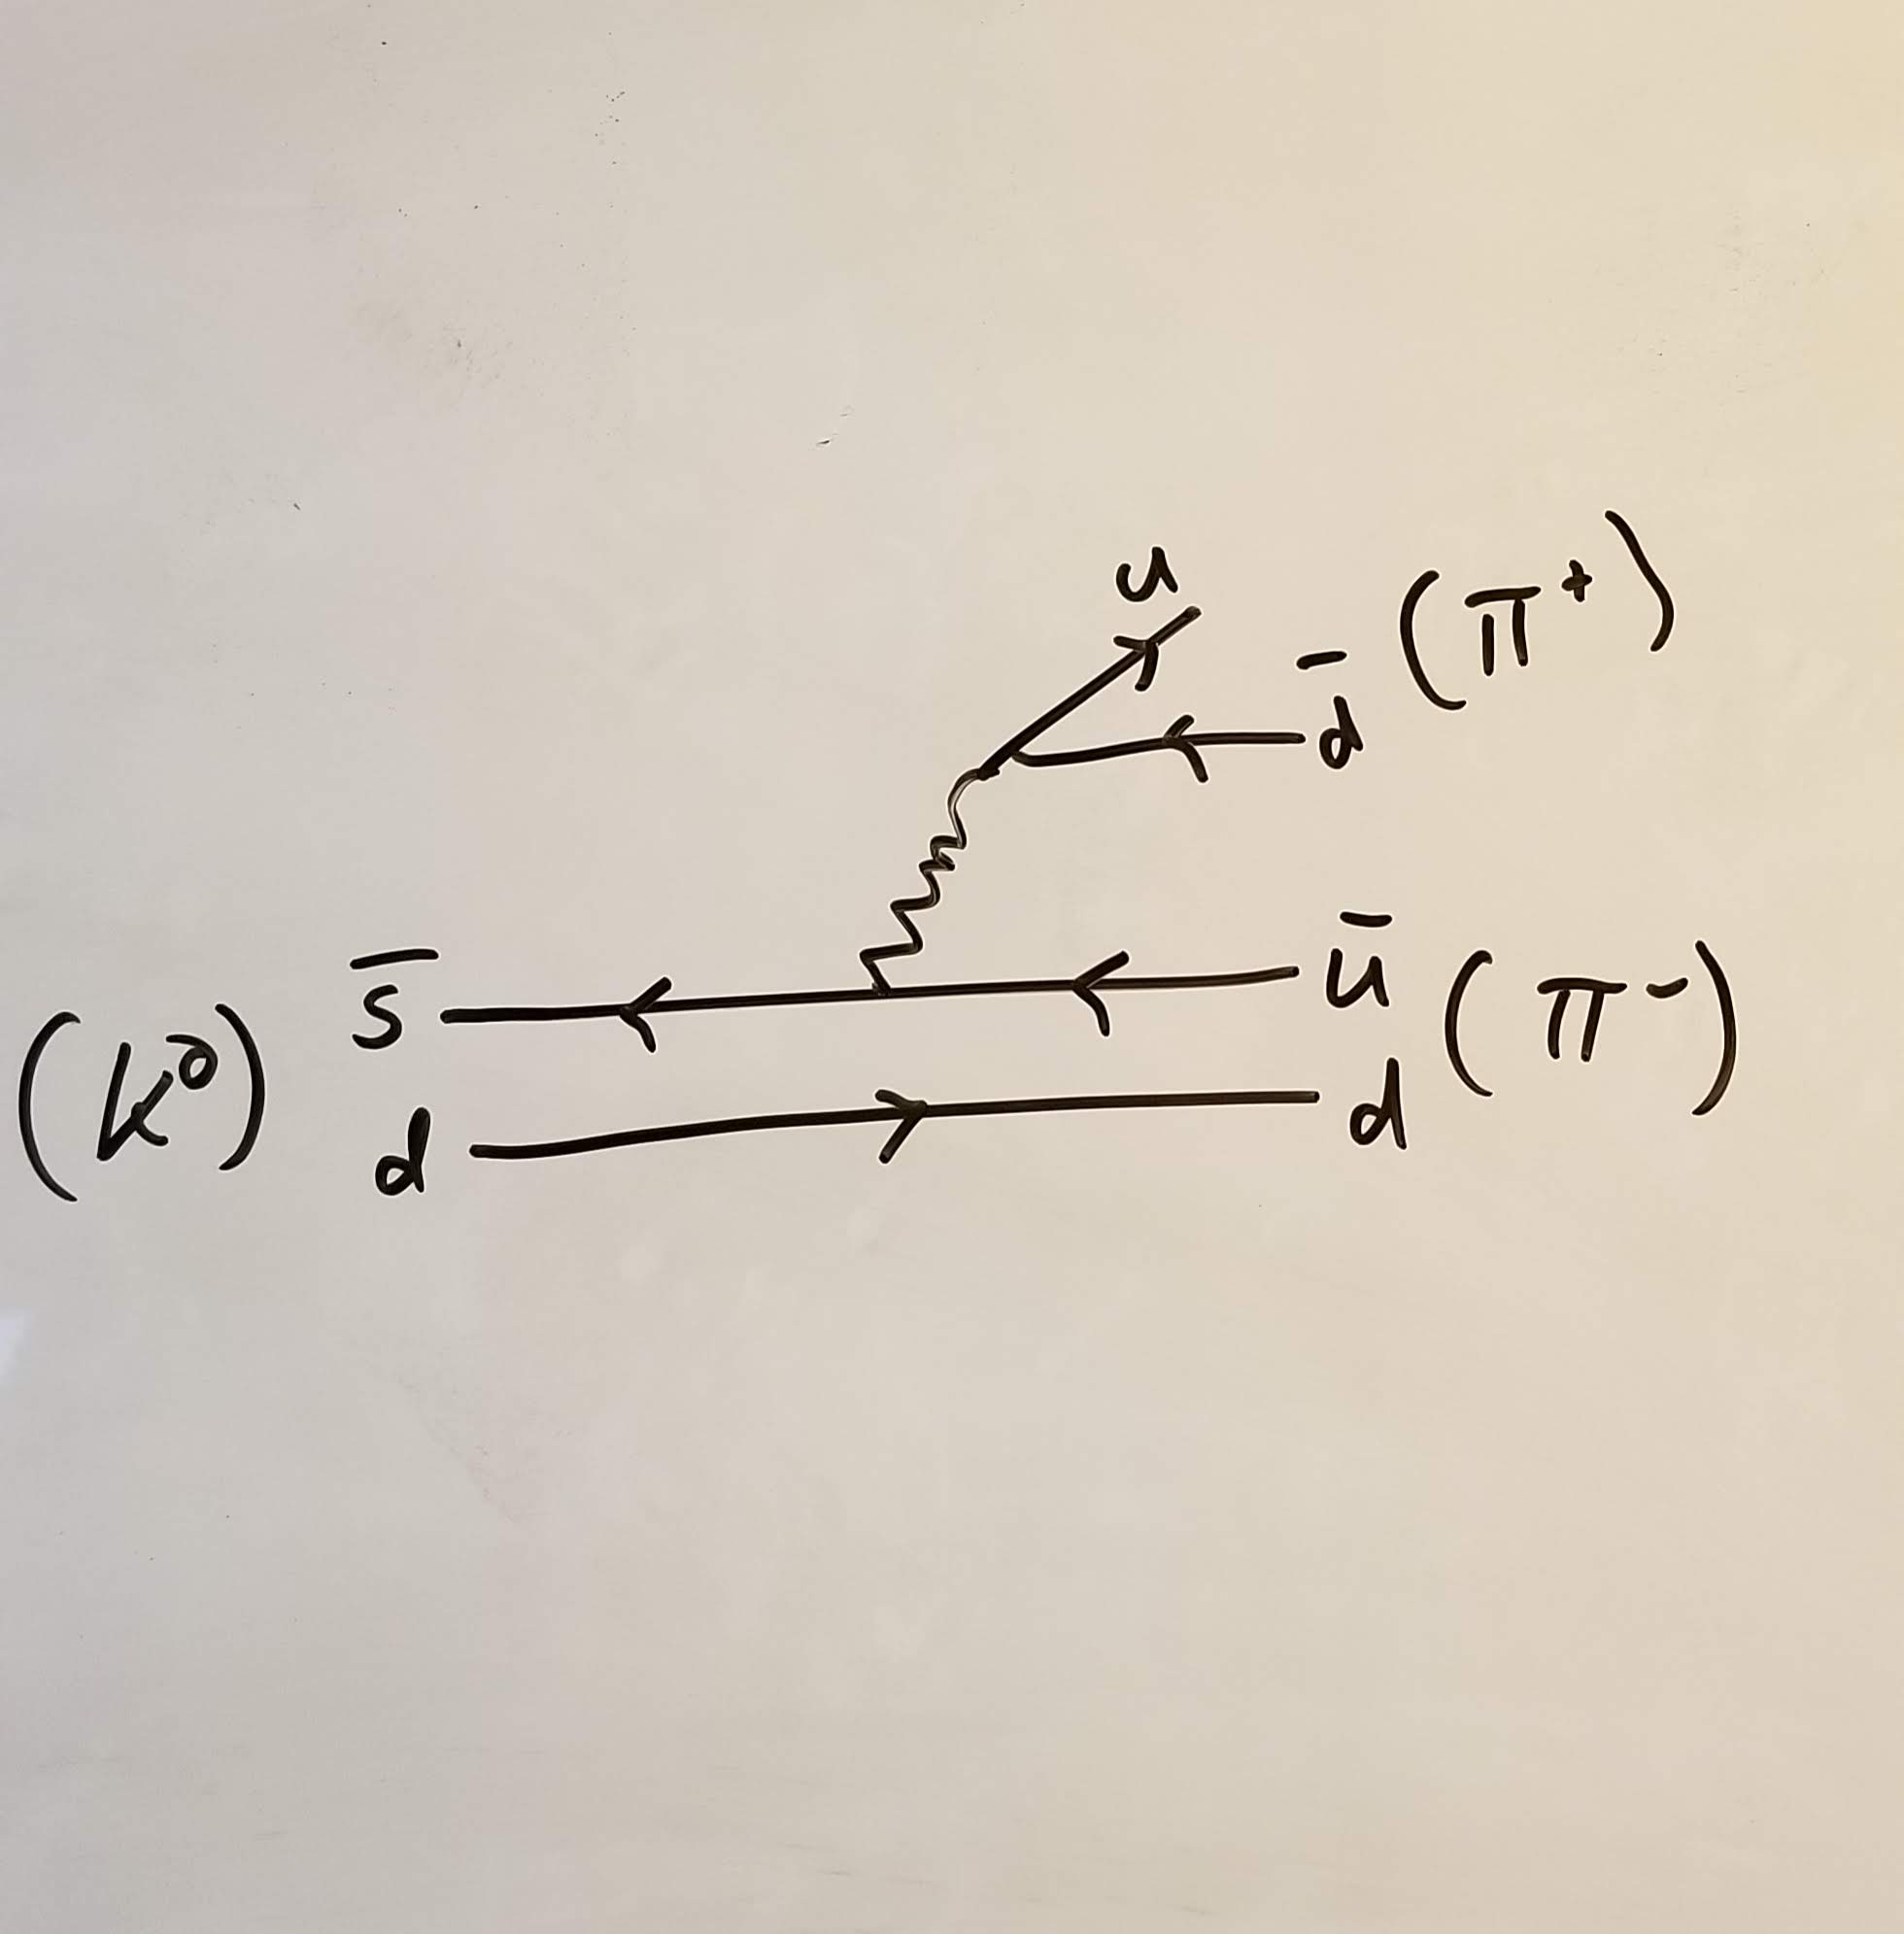
\includegraphics[scale=0.2]{k}
	\centering
	\caption{$K^0\rightarrow \pi^+\pi^-$}
	\label{}
	\centering
\end{figure}
\begin{figure}[h]			
	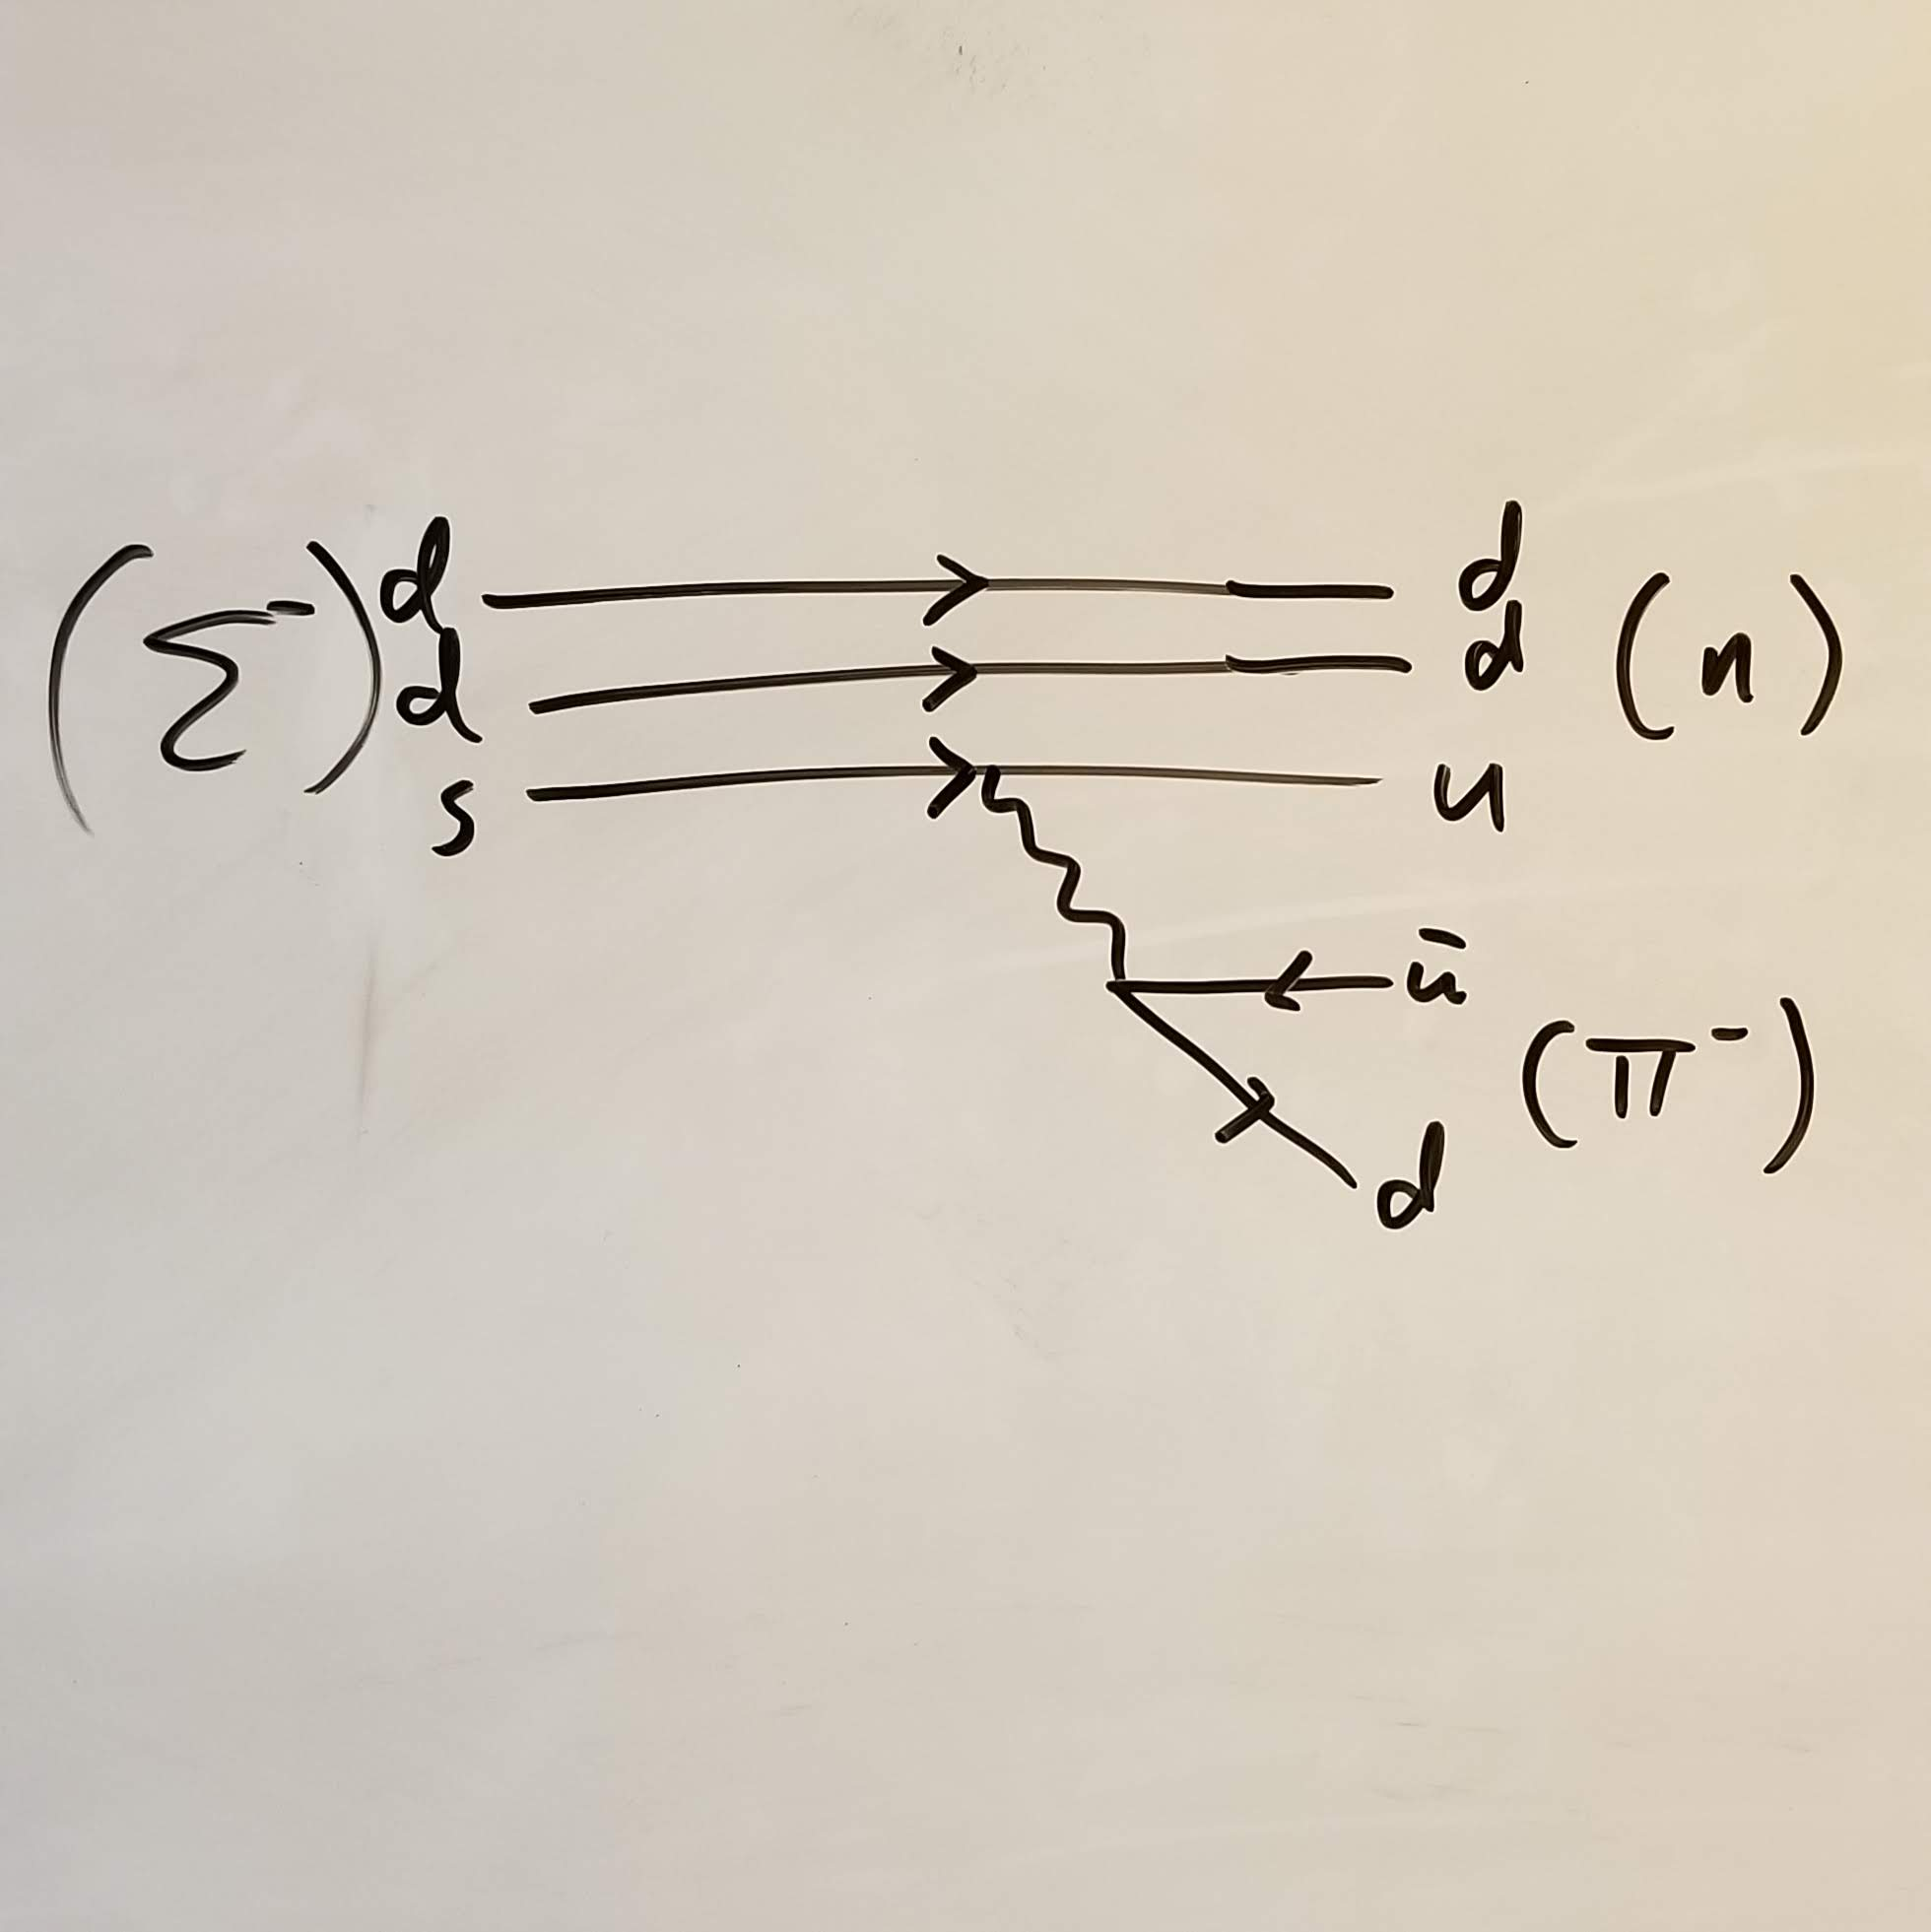
\includegraphics[scale=0.2]{sigma}
	\centering
	\caption{$\Sigma^-\rightarrow n\pi^-$}
	\label{}
	\centering
\end{figure}
\begin{figure}[h]			
	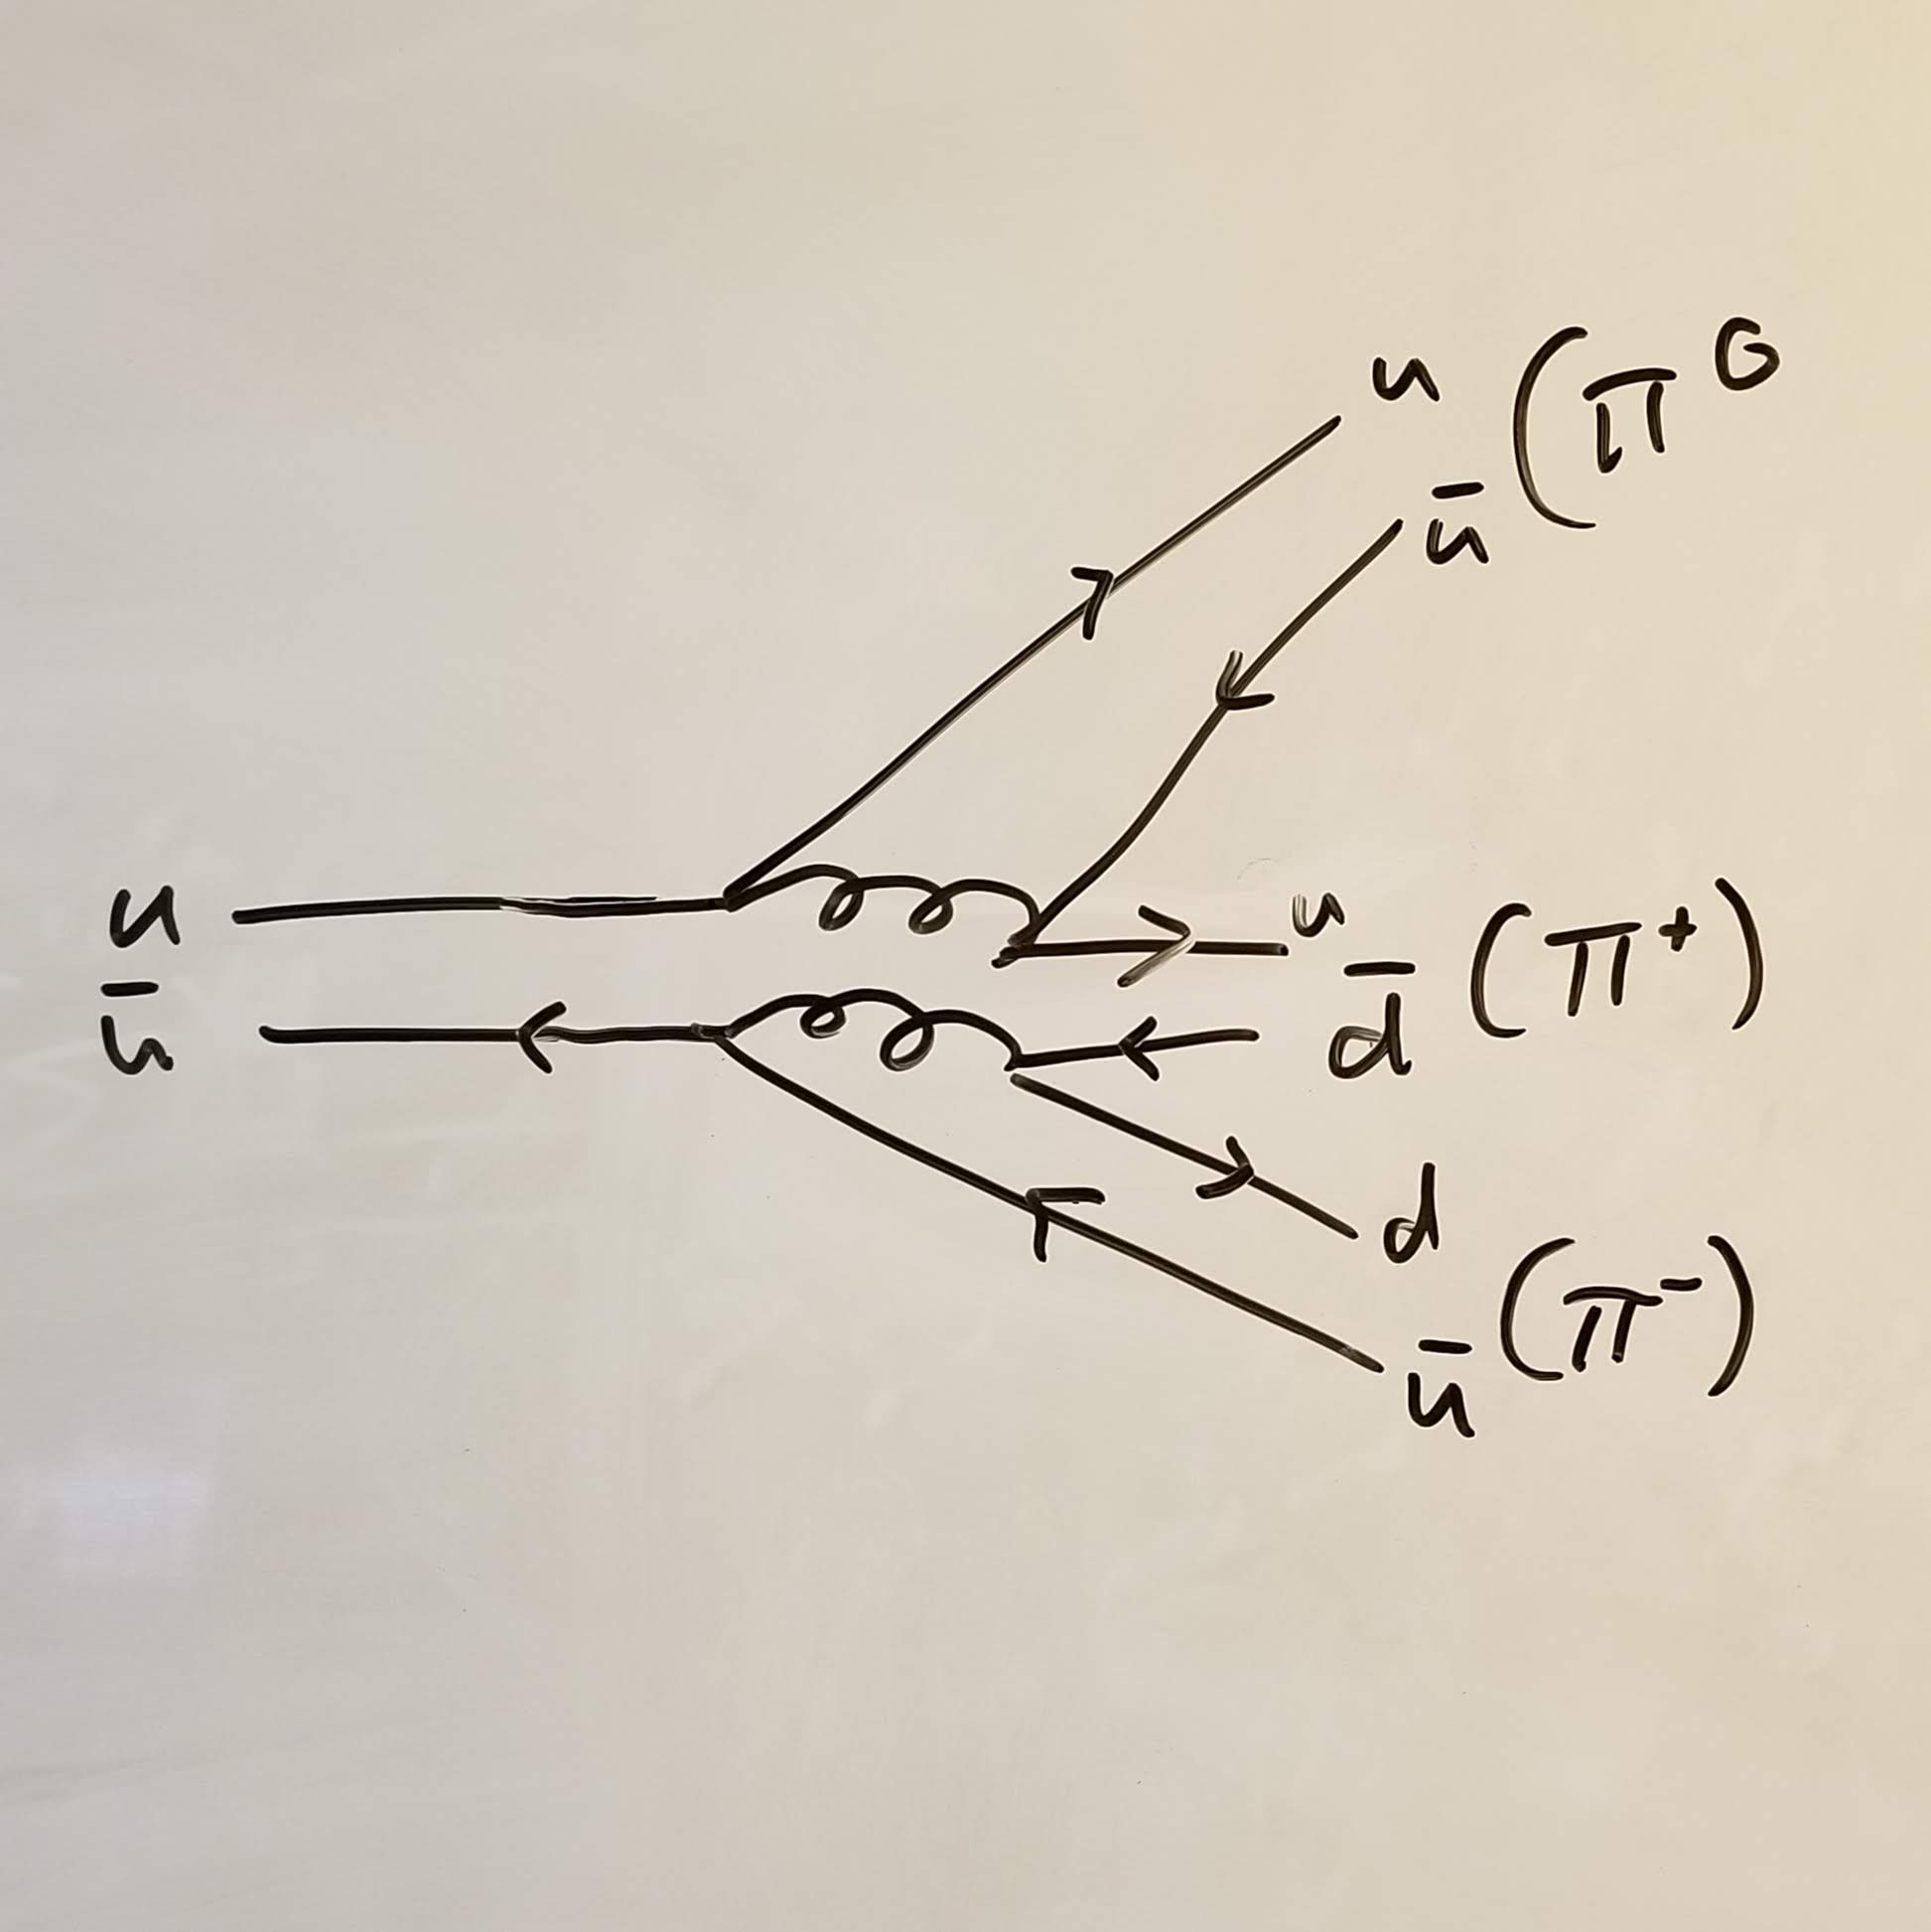
\includegraphics[scale=0.2]{omega}
	\centering
	\caption{$\omega^0\rightarrow \pi^+\pi^-\pi^0$}
	\label{}
	\centering
\end{figure}
\begin{figure}[h]			
	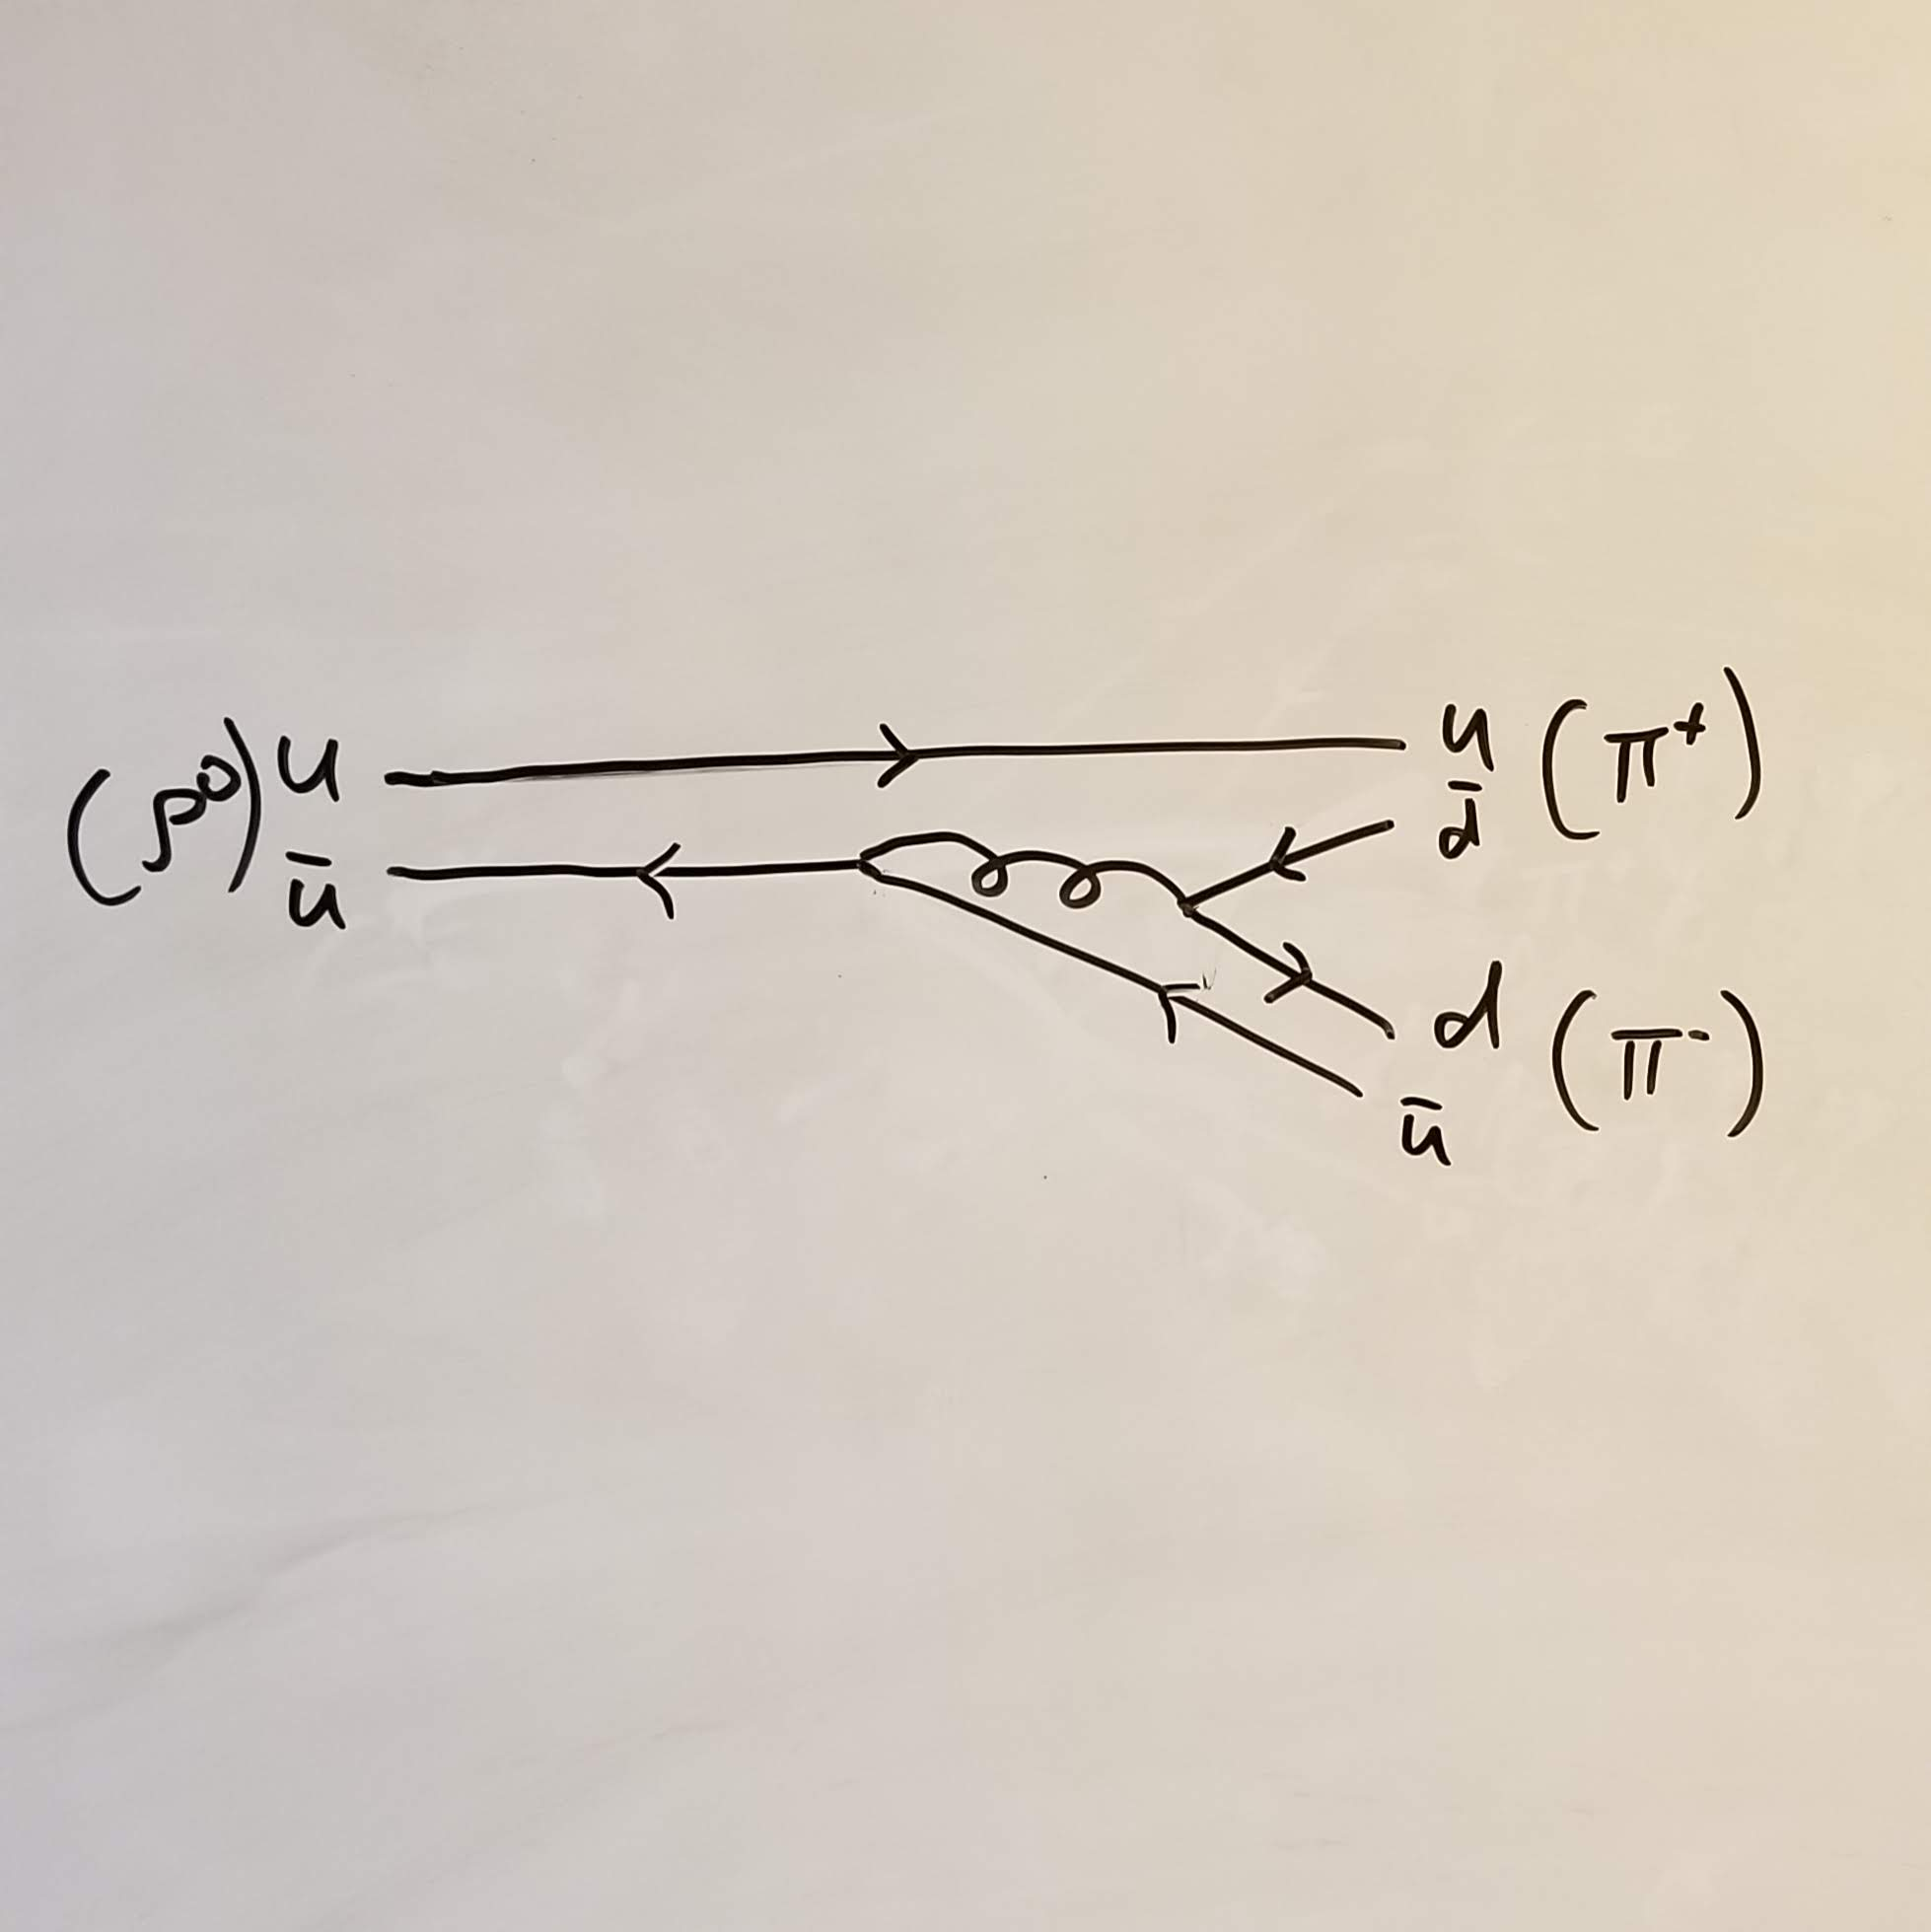
\includegraphics[scale=0.2]{rho}
	\centering
	\caption{$\rho^0\rightarrow \pi^+\pi^-$}
	\label{}
	\centering
\end{figure}
\begin{figure}[h]			
	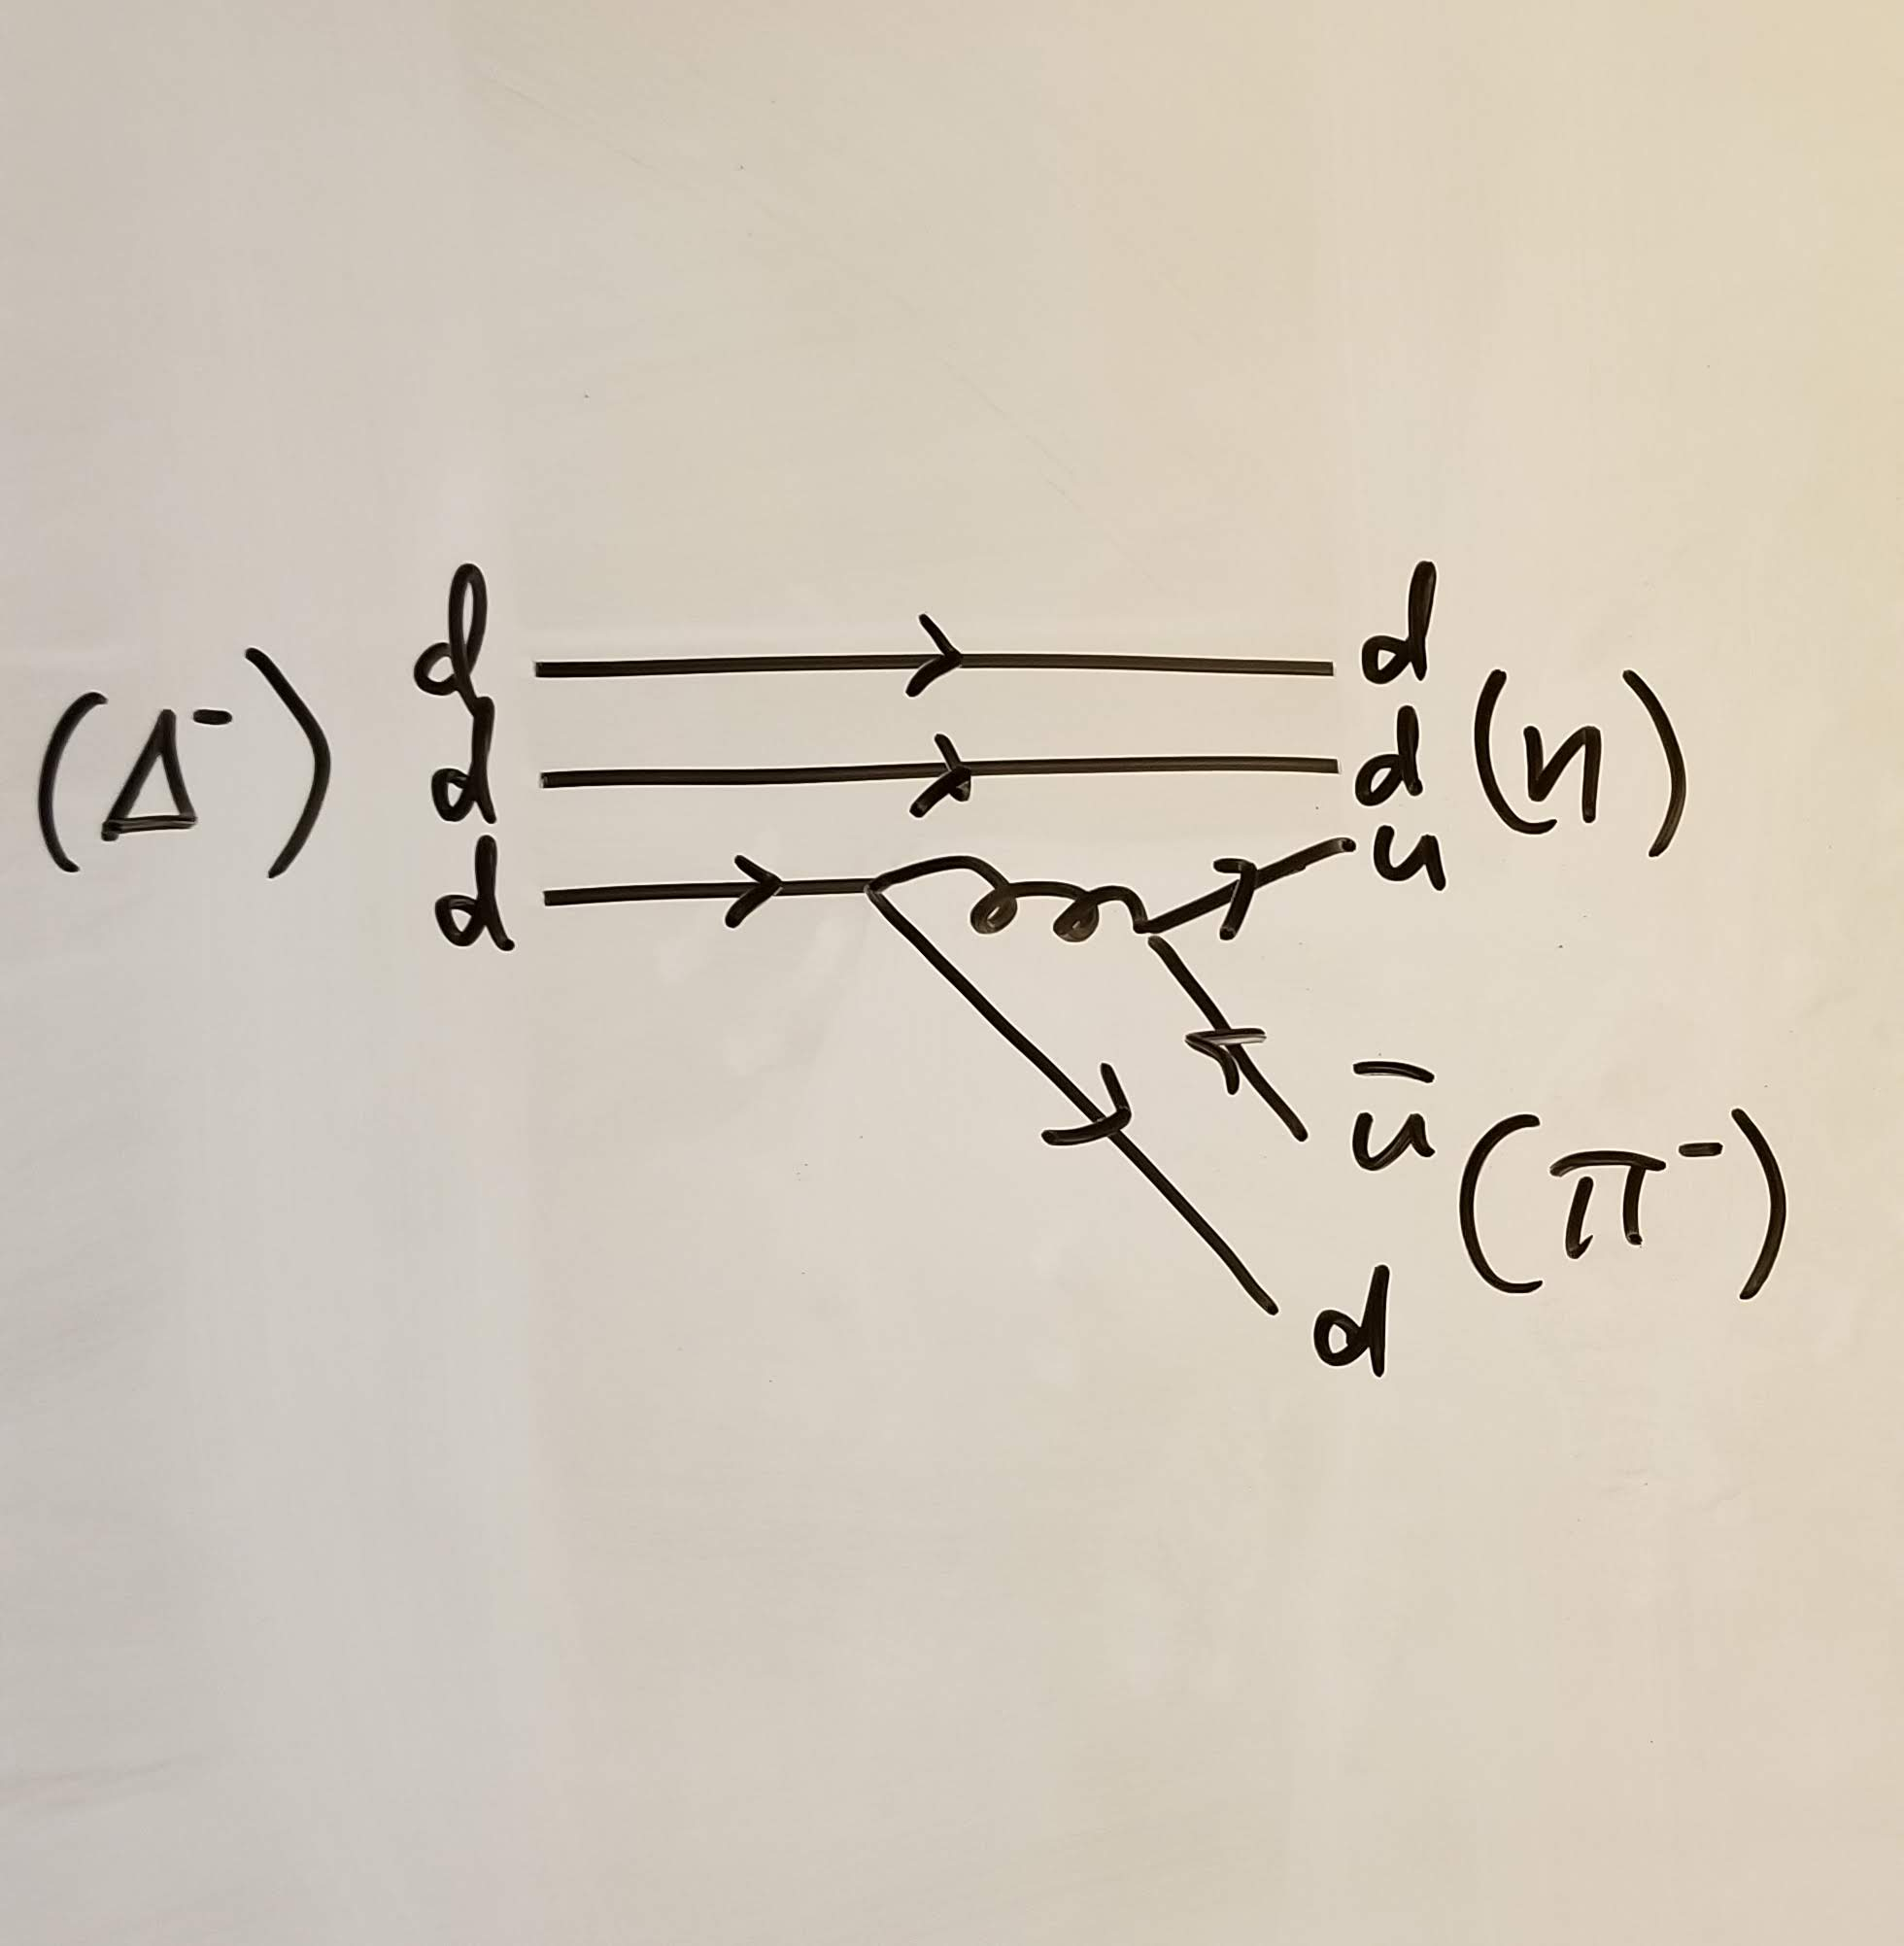
\includegraphics[scale=0.2]{delta}
	\centering
	\caption{$\Delta^-\rightarrow n\pi^-$}
	\label{end}
	\centering
\end{figure}

\end{homeworkProblem}

\pagebreak

\begin{homeworkProblem}
	Look up the branching ratios for the processes $K^+\rightarrow \pi^+\pi^-e^+\nu_e$ and $K^+\rightarrow \pi^+\pi^-e^-\bar{\nu}_e$. In both cases charge is conserved, so it seems that both decays should be possible. Can you explain what is going on?
	\\
	\\
\textbf{Solution}
\\
\\
If you look at Figure \ref{plot1}, you'll see a diagram with four vertices, two with strong coupling and two with weak coupling. But if you look at Figure \ref{plot2} you'll see a plot with six vertices, four of which are weak and two are strong. The additional weak couplings paired with the fact that one is a loop, means that this second diagram is highly suppressed.

\begin{figure}[h]			
	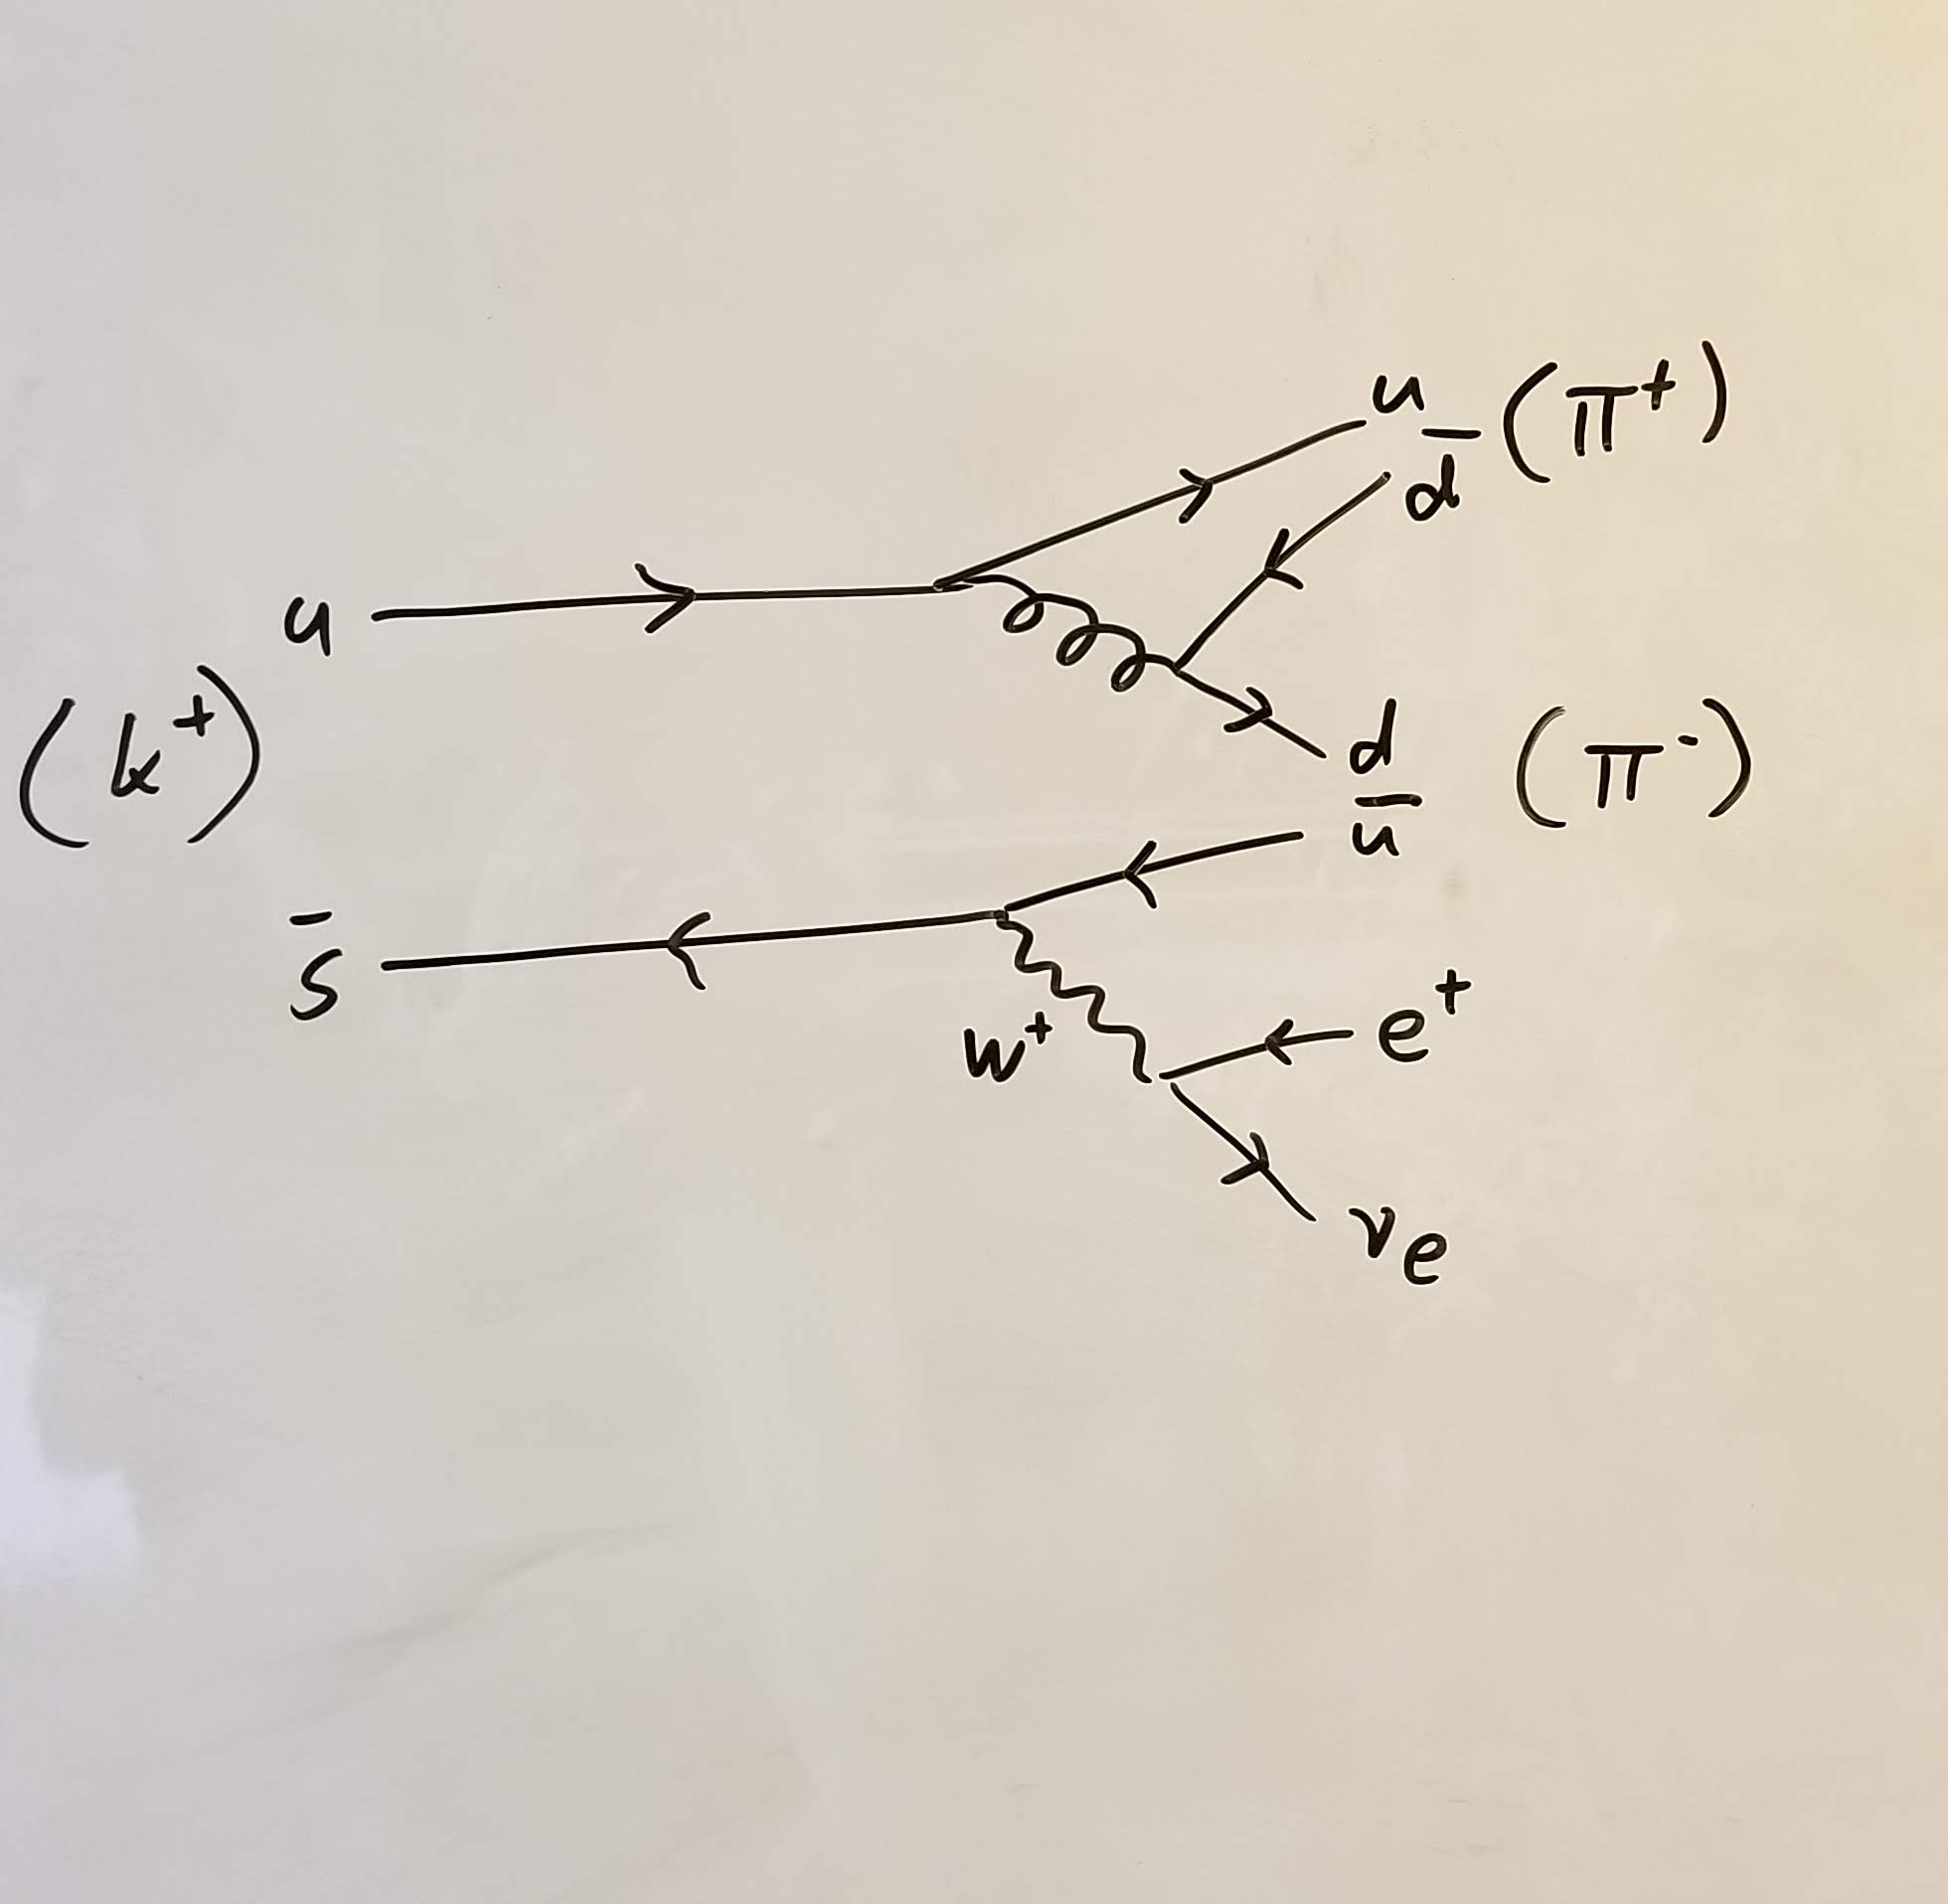
\includegraphics[scale=0.2]{pFour1}
	\centering
	\caption{$$}
	\label{plot1}
	\centering
\end{figure}
\begin{figure}[h]			
	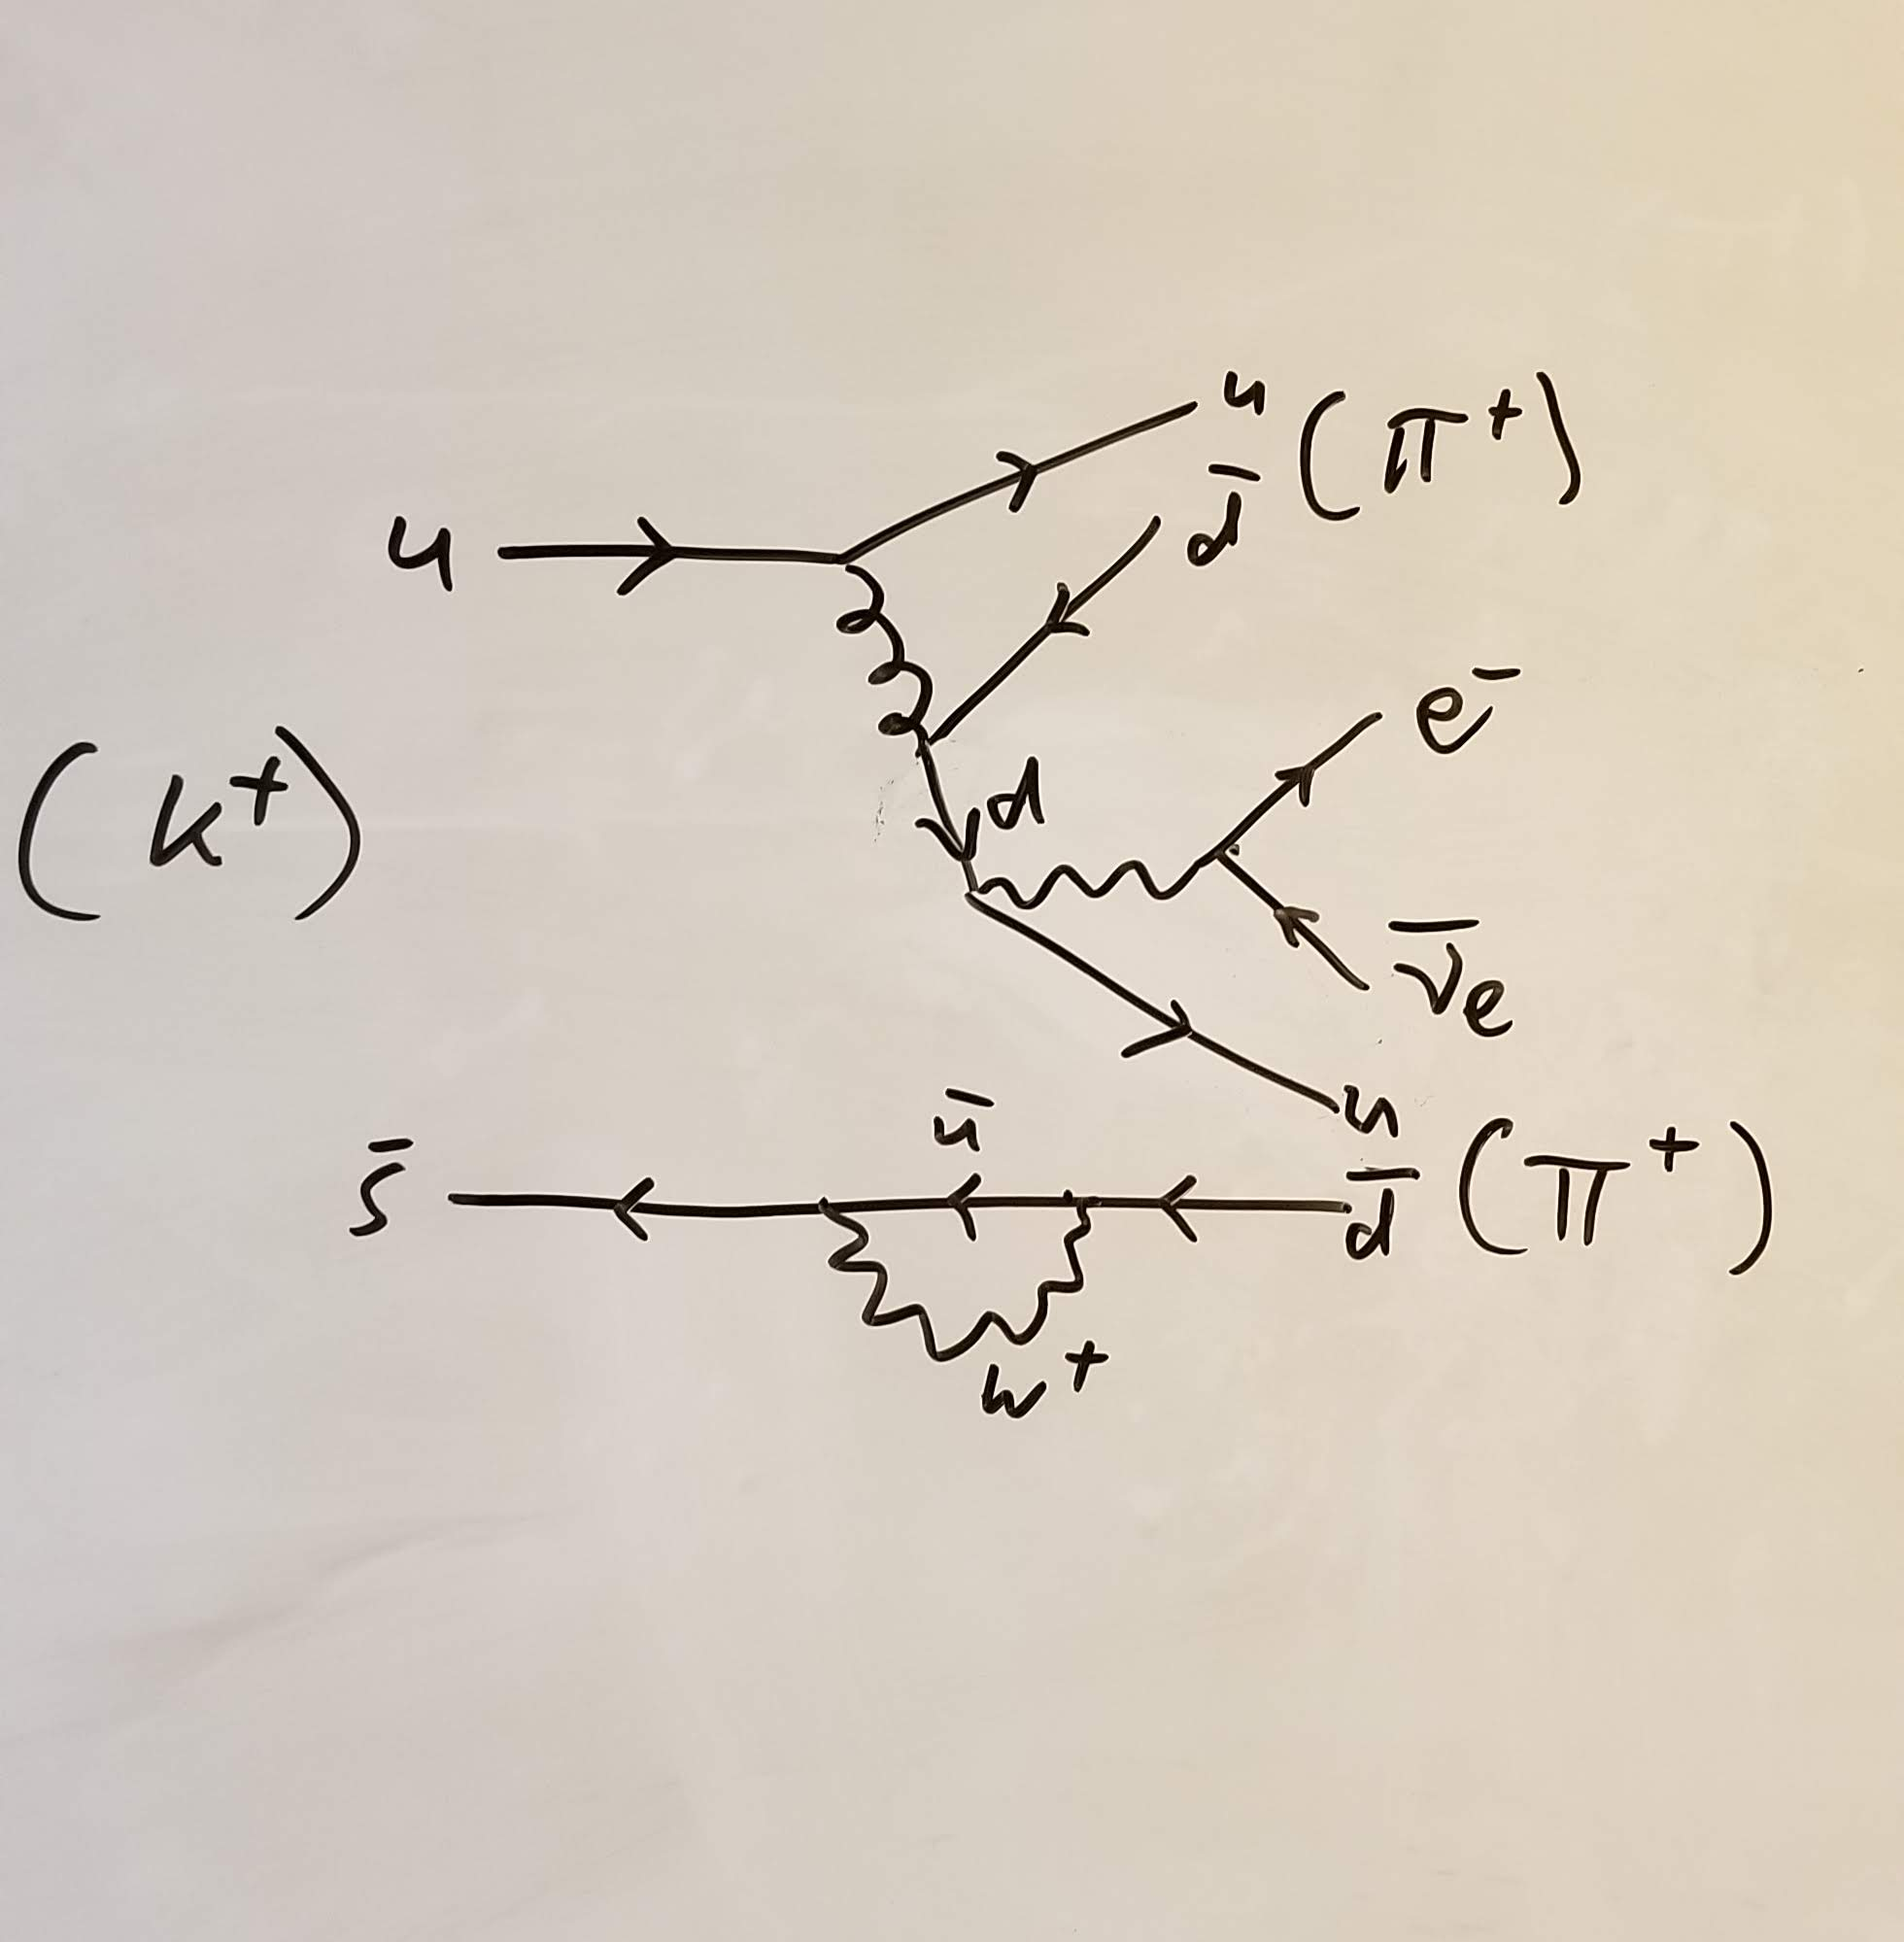
\includegraphics[scale=0.2]{pFour2}
	\centering
	\caption{$$}
	\label{plot2}
	\centering
\end{figure}
\end{homeworkProblem}

\pagebreak

\begin{homeworkProblem}
	In class, we talked about how the probability of decay $\Gamma$ is related to the particle lifetime $\tau=1/\Gamma$. But we had imagined only one possible decay mode for the particle. Now imagine that there are many different possible final states i of the decay. Then there is a probability $\Gamma_i$ for the decay to each of the final states.
	\\
	\\
	(a) What is the total decay probability in terms of $\Gamma_i$? What fraction of decays will be to a particular final state i?
	\\
	\\
	(b) What is the lifetime of the particle in terms of the $\Gamma_i$? As the number of possible decay modes increases, what happens to the lifetime?
	\\
	\\
	\textbf{Solution}
	\\
	\\
	(a) The total probability is the sum of the probabilities for every process:
	\[
		\Rightarrow \Gamma = \sum_{i}^{N}\Gamma_i
	\]
	Where there are N final states.
	\\
	\\
	The fraction into a particular state would be:
	\[
		\frac{\Gamma_i}{\Gamma}=\frac{\Gamma_i}{\sum_{i}^{N}\Gamma_i}
	\]
	(b)
	\\
	\[
		\tau=\frac{1}{\Gamma}=\frac{1}{\sum_{i}^{N}\Gamma_i}
	\]
	The more decay modes there are, the larger $\Gamma$ becomes since probabilities are always positive. This means that more decay modes means shorter overall lifetimes for the parent particle.
	
\end{homeworkProblem}

\pagebreak

\begin{homeworkProblem}
	To get ready for learning special relativity as it is used in particle physics, let's warm up with a review of undergraduate relativity. Consider two reference frames, S and S'. We establish coordinate systems in both frames with axes that are parallel to each other, and the z axis pointing in the direction of the relative motion of the two frames. S' moves in the +z direction with respect to S, with velocity v. Space-time displacements in the two frames are related by the Lorentz transformation,
	\begin{equation}
	\Delta x'=\Delta x
	\end{equation}
	\begin{equation}
	\Delta y'=\Delta y
	\end{equation}
	\begin{equation}
	\Delta z'=\gamma \Delta z-\beta \gamma c\Delta t
	\end{equation}
	\begin{equation}
	\Delta c\Delta t'=\gamma c\Delta t-\beta \gamma \Delta z
	\end{equation}
	where c is the speed of light in a vacuum, $\beta=v/c$ and $\gamma=1/\sqrt{1-\beta^2}$
	\\
	\\
	(a) A clock is at rest in S. An observer in S' sees the clock tick off $\Delta t'$ seconds. Use the Lorentz transformation to find how many seconds has ticked off in S.
	\\
	\\
	(b) A meter stick oriented along the z axis in S has length $\Delta z$. What is its length $\Delta z'$ in S'? 
	\\
	\\
	(c) Let the differential element $\Delta x, \Delta y, \Delta z, \Delta t$ describe the motion of a photon. The photon has speed c in the frame S. By construction, we must have
	\begin{equation}
	\sqrt{(\Delta x)^2+(\Delta y)^2+(\Delta z)^2}-c\Delta t=0
	\end{equation}
	Use the Lorentz transformation to evaluate the similar expression in S'. Note an important implication of your result - the left hand side of the equation will have the same value no matter what frame it is evaluated in, even if it has a non-zero value.
	\\
	\\

	\textbf{Solution}
	\\
	\\
	(a) For a clock at rest in S, $\Delta z=0$
	\[
		\Rightarrow \Delta t' = \gamma \Delta t
	\]
	In the frame S, \(\Delta t = \Delta t'/\gamma\) seconds have ticked.
	\\
	\\
	(b) Measuring simultaneously implies that $\Delta t'=0$
	\[
		\begin{split}
		\Rightarrow \Delta z = \gamma \Delta z'\\
		\Rightarrow \Delta z' = \frac{1}{\gamma}\Delta z
		\end{split}
	\]
	(c) Square both sides ot make this neater
	\[
		(\Delta x)^2+(\Delta y)^2+(\Delta z)^2=c^2(\Delta t)^2
	\]
	Carry out the inverse transformations:

	\[
		\begin{split}
		(\Delta x')^2+(\Delta y')^2+(\gamma\Delta z'+\beta\gamma c\Delta t')^2\\
		=(\gamma c\Delta t'+\beta\gamma\Delta z')^2 \\
		(\Delta x')^2+(\Delta y')^2+\gamma^2(\Delta z')^2+\beta^2\gamma^2c^2(\Delta t')^2 +2\gamma^2\beta c\Delta z'\Delta t' \\
		= \gamma^2c^2(\Delta t')^2+\beta^2\gamma^2(\Delta z')^2+2\gamma^2\beta c \Delta z'\Delta t' \\
		(\Delta x')^2+(\Delta y')^2+\gamma^2(\Delta z')^2-\beta^2\gamma^2(\Delta z')^2+\beta^2\gamma^2c^2(\Delta t')^2-\gamma^2c^2(\Delta t')^2=0 \\
		(\Delta x')^2+(\Delta y')^2+\gamma^2(\Delta z')^2(1-\beta^2)-\gamma^2c^2(\Delta t')^2(1-\beta^2)=0
		\end{split}
	\]
	But recall that \((1-\beta^2)=1/\gamma^2\)
	\[
		\begin{split}
		\Rightarrow (\Delta x')^2+(\Delta y')^2+(\Delta z')^2=c^2(\Delta t')^2 \\
		\sqrt{(\Delta x')^2+(\Delta y')^2+(\Delta z')^2}-c\Delta t'=0
		\end{split}
	\]

\end{homeworkProblem}

\end{document}
